This chapter discusses the evaluation of the \ce{BrO} SCD , calculated from the spectra recorded by the spectroscopic instruments of NOVAC. The BrO SCD error hereby taken as a measure for the quality of the BrO retrieval.\\
\Cref{fig:allbroerrordistribution} shows the BrO "Multi Add"\footnote{More information about the multiadd-retrieval and the fit settings can be found in \Cref{Chap:evalroutine}} retrieval error distribution, which is centered around $1.1\cdot10^{+13}$ to $1.4\cdot 10^{+13}\frac{molec}{cm^2}$. \\
\\
The evaluation of the data from NOVAC are separated in the evaluation of \ce{SO2} and the evaluation of BrO. While the retrieval of \ce{SO2} is relatively easy due to the high amount of \ce{SO2} in the plume (magnitude of \ce{SO2} at Tungurahua $\approx 1\cdot 10^{18}$), the \ce{BrO} evaluation is much more challenging due to not distinct BrO curves as a result of the lower BrO magnitudes (as can be seen in \Cref{fig:plumeref}). The magnitude of \ce{BrO} SCD is around $\approx 1\cdot 10^{14}\frac{molec}{cm^2}$. \\
%
\begin{figure}
	\subfigure{
		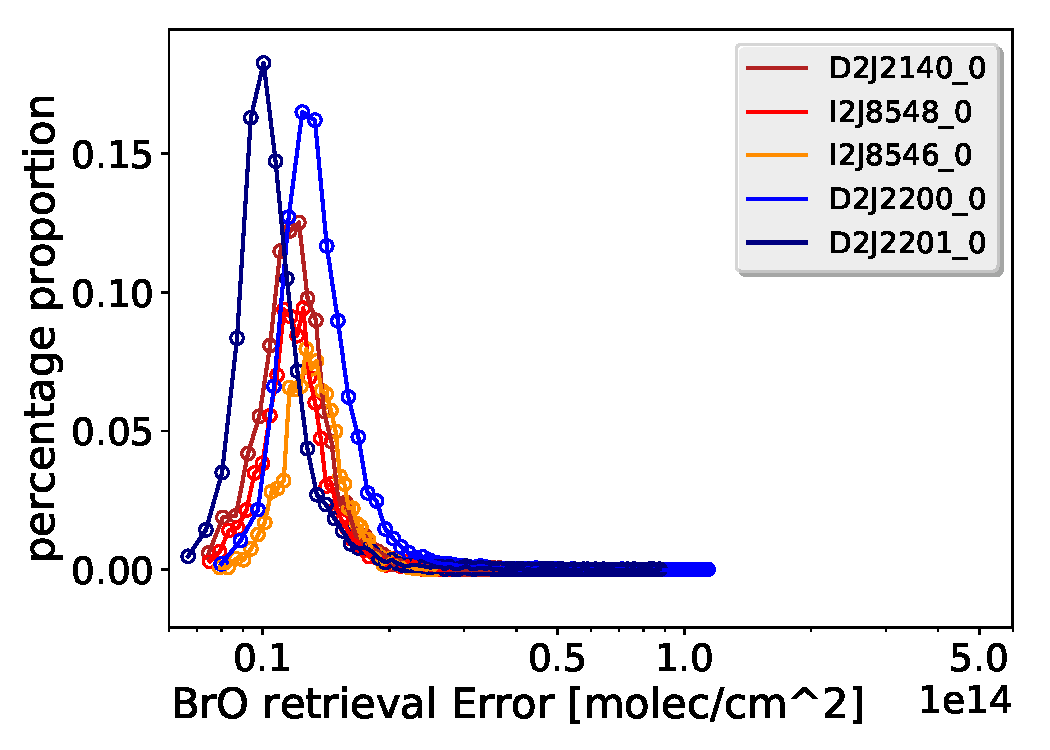
\includegraphics[width=0.49\linewidth]{Bilder/sametimeBrOErrorDistribution}}
	\subfigure{
		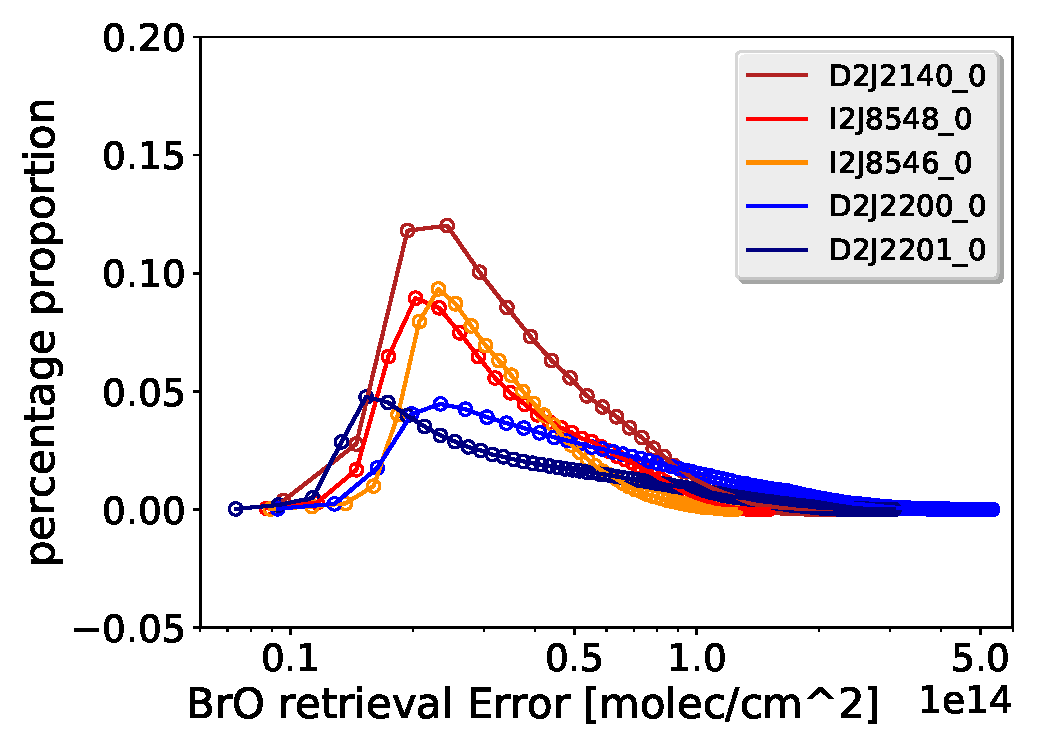
\includegraphics[width=0.49\linewidth]{E:/Masterarbeit/BrO_Error_Distribution/AllBrOErrorDistribution}}
	\caption{Histogram of \ce{BrO} error, shown for all instruments considered in this thesis. Left: The \ce{BrO} distribution for the "same time retrieval".Right: The \ce{BrO} error distribution for the evaluation with a reference from another time, where the temporal difference between plume and reference is not longer that two weeks. The instruments of Nevado del Ruiz are coloured blue, while the the instruments of Tungurahua are coloured in yellow to red.
		The peaks for the single instrument are located at: D2J2140: 1.2$\cdot 10^{13}\frac{molec}{cm^2}$; I2J8548: 1.3$\cdot 10^{13}\frac{molec}{cm^2}$;
		I2J8546: 1.4$\cdot 10^{13}\frac{molec}{cm^2}$;
		D2J2200: 1.4$\cdot 10^{13}\frac{molec}{cm^2}$;
		D2J2201: 1.1$\cdot 10^{13}\frac{molec}{cm^2}$}
	\label{fig:allbroerrordistribution}
\end{figure}
%
This results in a larger uncertainty of the \ce{BrO}  SCD. Most of the \ce{BrO} data (98.3\% of the data) are below the detection limit of \ce{BrO}$_{err}$/\ce{BrO}$_{value}$<1/4. Hereby is \ce{BrO}$_{err}$ the BrO fit error, and \ce{BrO}$_{value}$ the BrO SCD. In comparison SCDs of \ce{SO2} in almost all cases (99.5\% of the data)  are above the detection limit. \\
%
Choosing a different reference spectrum than the reference measured at the same time as the plume in 99\% of all possible cases results in an increasing of the absolute error. 
It is expected that the evaluation with an alternative spectrum results in general in a higher BrO error than when evaluated with the same time spectrum.\\
However, for a contaminated same-time-reference the relative error might decrease due to the underestimation of the gas amount. \\
Due to the large uncertainty of \ce{BrO} relative to \ce{SO2} the optimization of the \ce{BrO} error is of particular importance. Therefore, the reference is chosen with respect to the \ce{BrO} error to maximize the quality of the \ce{BrO}/\ce{SO2} ratio. \\
\\
The amount of gas free alternative references is around 1500 per year. To make an optimal choice, it is necessary to examine the conditions which influence the \ce{BrO} retrieval.\\
Every spectrum is recorded under particular/unique ambient conditions. These measuring conditions generally are not equal for different scans. In this study, I show that references for which the surrounding conditions e.g temperature or cloudiness are similar with the surrounding conditions of the  plume measuring lead to a smaller error.\\
%
\subsubsection*{Data used for the analysis}
I evaluate a fixed plume spectrum using more than 1000 recorded multi add reference spectra in order to find the optimal reference spectrum. This evaluation is performed for more than 1000 multi add plume spectra in order to obtain a high statistical significance. Thus 1000 recorded multi add spectra result in $1000^2$ possible plume reference pairs and the corresponding differences in the external parameter and their associated \ce{BrO} error. 


\section{Influence of ambient conditions on the measurement \label{Chap:BROErr}}
The measurement and evaluation of the spectra monitored with NOVAC depends on the ambient conditions like temperature or cloudiness \citep{lubcke2014optical}.\\
Thus, the ambient conditions need to be taken into account for choosing a new reference.\\
The analysis of these external parameters are performed for spectra recorded at Tungurahua and Nevado del Ruiz. At Tungurahua three instruments (I2J8548; D2J2140; I2J8546) with data recorded in the time span from July in 2008 to August in 2009 are used. Nevado del Ruiz contributes with two instruments (D2J2200; D2J2201) in the time from the end of 2009 to the end of 2011.\\
%
The ambient conditions that are considered in this thesis are:
\begin{table}[h!]
	\centering
	\fbox{\begin{tabular}{p{4cm}p{8.5cm}}
		%	\toprule
		Temporal difference &Temporal difference between measuring the plume and the reference.\\
		Daytime & Time of the day, and thus a measure of solar altitude.\\
		Temperature& The temperature of the instrument while recording the spectra.\\
		Colour index&Ratio of two intensities at different wavelength as a measure for the cloudiness of the sky.\\
		Exposure time& Length of time the sensor of the NOVAC instrument is exposed to light.\\
		Elevation angle& Orientation of the instrument relative to the zenith, which corresponds to an elevation angle of zero degree.\\
		\label{tab:externalparametters}
	\end{tabular}}
\end{table}	
%



\subsection{Statistical assessment scale}

The external parameters described above are analysed one by one in the following sections. Hereby I will proceed as follows:
A first step is to define a maximal temporal difference to prevent too large computational time.\\
The BrO measurement error as a function of the difference in the specific external parameter between the reference spectrum and the plume spectrum is shown for each of the individual instruments at Tungurahua and Nevado del Ruiz. 
To quantify the dependency between the BrO retrieval error and the external parameter, the data are fitted with a first order polynomial for each of the individual instruments at Tungurahua and Nevado del Ruiz. Hereby only the absolute differences were used. For every external parameter the fitting parameters slope and intercept are calculated.\\
Moreover, the correlation(See site \pageref{ff})  between the BrO fit error and the absolute difference in the specific external parameter is calculated. If the BrO retrieval increases with increasing differences in surrounding condition between the plume spectra and the reference spectra, the difference, where the BrO retrieval error $Mean(\Delta EP_{2})$\footnote{EP: placeholder for any external parameter} is twice as high as for no difference is also calculated.\\  
Differences in external parameters can lead to large uncertainties in the retrieval, thus I analyse the amount of data possible references, if only data with differences smaller than $Mean(\Delta EP_{2})$ in the specific external parameter are used. 
The advantage of restricting the accepted difference between the plume and the reference spectrum is a better control of the choice of the best reference. The disadvantage is that the amount of possible references decreases. Thus, it could occur that a reference is dismissed, which has a large difference in one parameter but is very similar in the remaining parameters.\\
The Mean, the corresponding standard deviation as well as the minimum and the maximum amount of references are calculated for each instrument.
\begin{center}
	\label{ff}
	\fbox{\parbox{13cm}{The Correlation coefficient $\rho_{X,Y}$ used in this thesis refer to the pearson product-moment correlation coefficients. It is a measure of linear correlation between two variables X and Y. The pearson correaltion coefficients range from -1 to +1.  Where +1 is total positive linear correlation,  -1 describes a total negative linear correlation, and a correlation of 0 refers to no linear correlation. The formula for the correlation coefficient is:
			\begin{equation*}
			\rho_{X,Y}=\frac{cov\left(X,Y\right)}{\sigma_X\sigma_Y}
			\end{equation*}
			were:
			$cov$  is the covariance\\
			$\sigma_X$ is the standard deviation of X\\
			$\sigma_{Y}$ is the standard deviation of Y\\
			Here the correlation is computed using the python\footnote{version 2.7.1} library Numpy (version 1.5.6)}}
	
\end{center}
%	
\subsection{Temporal difference}
%
\begin{figure}
	\centering
	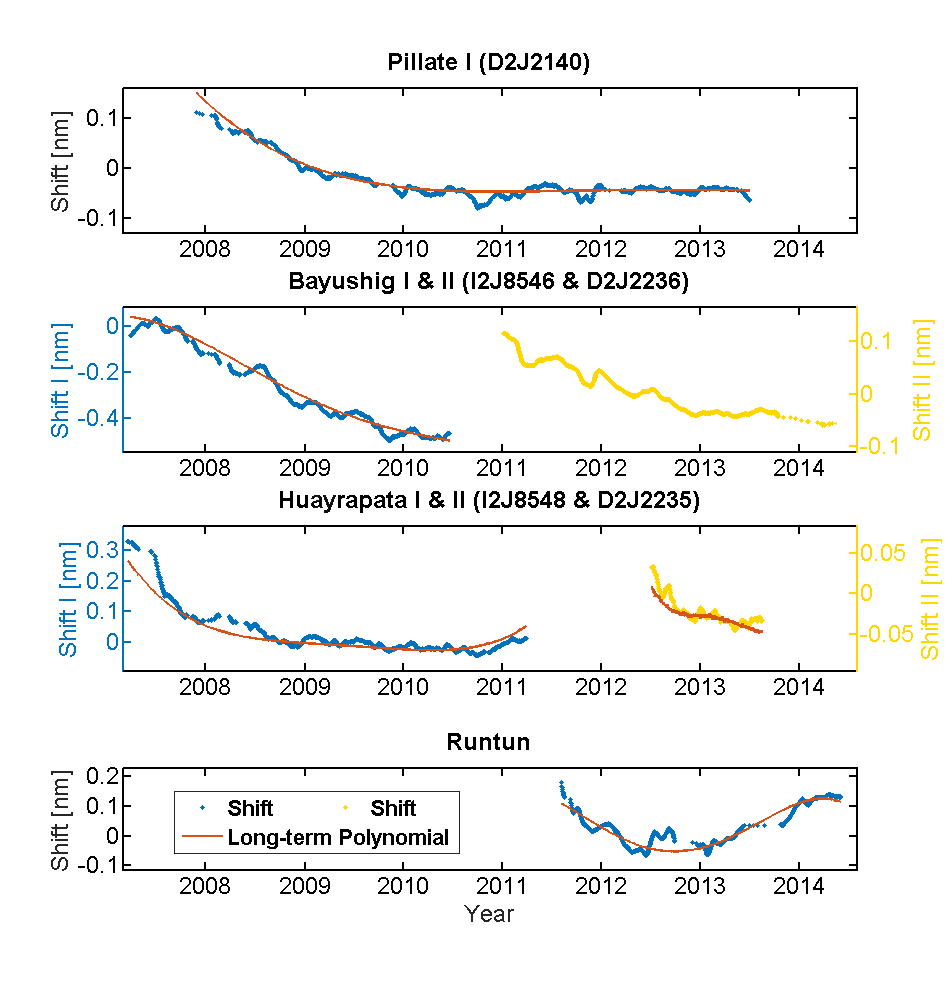
\includegraphics[width=1\linewidth]{Bilder/Simon/Bilder_Tung/Drift_Komplett_NEW}
	\caption{Wavelength shift over the time. The shift is shown for six NOVAC- instruments from Tungurahua. The red and yellow dots show the running mean over 20 days. Red line indicates a temperature independent long term polynomial. Source: \cite{WarnachSimon}}
	\label{fig:driftkomplettnew}
\end{figure}
%
\begin{figure}
	\subfigure[]{
		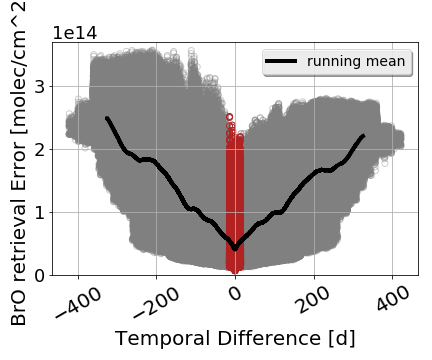
\includegraphics[width=0.5\linewidth]{Bilder/Datum}}
	\subfigure[]{
		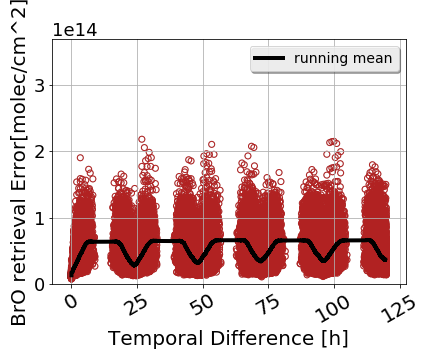
\includegraphics[width=0.5\linewidth]{Bilder/datumkurz}}	
	\caption{The \ce{BrO} error as a function of the temporal difference shown for the Pillate instrument from Tungurahua (2008-2009). The running mean is plotted with a black line. (a) Temporal differences up to 400 days. (b) Absolute temporal differences up to $\pm$ 120h. The periodical \ce{BrO}  error evolution indicates the impact of the daytime. }
	\label{fig:dat}
\end{figure}
%

Variation in the ambient conditions cause a temporal variation if the instrument response function/cause an instrumental drift. This could a result of the same changes which lead to the wavelength shift over time observed by \citet{WarnachSimon}.  \citet{WarnachSimon} suggests that the drift is caused by a hysteresis effect. \Cref{fig:driftkomplettnew} shows the wavelength shift as a function of the time for six NOVAC instruments located at Tungurahua in the time between 2008 to 2014. \Cref{fig:driftkomplettnew} shows a rather steep drift in this time interval.
\citet{WarnachSimon} observed a decrease of the shift after initial negative drift after the first two years at Pillate station. Thus an rather step drift at new installed instruments can be observed. Therefore, it is observed that the temporal difference becomes less important after an initial adaptation on the surroundings after the installation of the instruments.\\
When using reference and plume spectra of the same time, these effects are cut out since the shift is equal for the plume and reference spectrum.\\
To examine the effect of the temporal difference on the retrieved \ce{BrO} error, for all reference-plume pairs the corresponding \ce{BrO} error is calculated. Due to the large amount of reference plume pairs within one year, it takes more than a month (Hardware details: Intel(R) Core(TM) i5-4570 CPU @ 3.20Ghz 64 Bit operating system, amount of 4 kernels) to evaluate the corresponding \ce{BrO} error for every possible reference-plume pair of one instrument. I did this for the  D2J2140 instrument installed at Tungurahua:\\
With the data from the D2J2140 instrument the dependency between the BrO retrieval error and the temporal difference between measuring the plume spectrum and the reference spectrum.\\
For an increasing temporal different between reference and plume measurement time the fit quality decreases on the average (On short timescales the influence of the temperature, daytime or other external parameter could be counteractive to the impact of the temporal distance). Thus a large temporal difference results in an increase of the \ce{BrO}  error of more than 600\% (see \cref{fig:dat} (a)).
\ce{BrO} errors of such magnitudes are too large for our purposes. Therefore, it is useful to set a maximal temporal difference, to prevent too large \ce{BrO} error and to reduce the calculation time.
%
In \cref{fig:dat} (a) it can be seen that the evolution of the \ce{BrO}  error with the temporal difference is symmetric around zero. Thus it is not necessary to distinguish between positive or negative temporal differences.
%The maximal temporal difference should be large enough to ensure a sufficient amount of references to be able to pick a reference with similar conditions. However, the maximal temporal difference should be small enough to prevent too large \ce{BrO} errors due to long term shifts.\\
\\
To evaluate the maximal time difference, for which the results are still reliable for every plume, where the "same time reference" is contaminated, the alternative reference is chosen, which leads to the minimal \ce{BrO} error.\\
% histogram
\begin{figure}
	\centering
	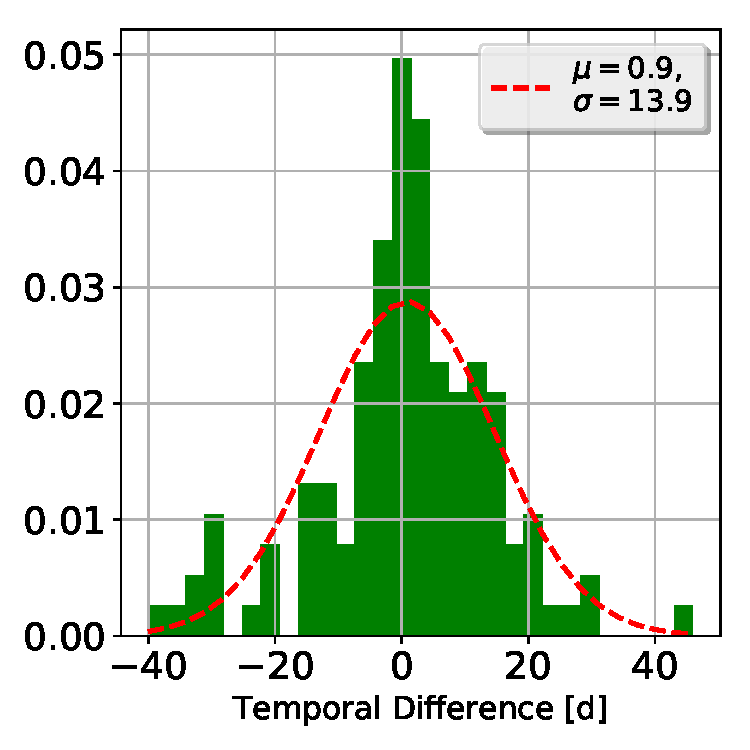
\includegraphics[width=0.6\linewidth]{Bilder/Hist}
	\caption{Histogram showing the frequency of getting the best reference as function of the temporal difference between plume and reference measuring. The temporal difference is negative if the reference spectrum was recorded after the plume spectrum. A Gaussian-like distribution is retrieved. The red dotted line visualizes a Gaussian fit for the shown histogram. The mean $\mu$ of the gaussian curve is: $\mu = 0.9$, the variance $\sigma$ is: $\sigma = 13.9$. The width of the green bars is three days.}
	\label{fig:Hist}
\end{figure}
%
In \cref{fig:Hist} a histogram with the probability of picking the best reference as a function of the time difference is plotted. The mean of the Gaussian fitted on the data is slightly above zero. However the variance is calculated as approximately 14 days, thus a mean of 0.9 is statistical irrelevant. To simplify the evaluation, and for a better traceability the absolute maximal temporal difference between the recording time of the reference and the plume spectrum should be equal for references recorded before and after the plume. For the retrieval all time differences are allowed within one sigma area. Thus, the maximal time difference is about two weeks.\\

% remaining possible reference spectra

	\begin{table}[h]
	\centering
		\caption{Amount of possible references when restricting the time span between plume and reference to two weeks. Here in the ”Mean” and “Std” row for each  instrument the average restriction is shown with the corresponding standard deviation. The “Min” and “Max” rows show the extend of restriction in the extreme cases.}
	\fbox{\begin{tabular}{p{1.8cm}p{2.15cm}p{2.15cm}p{2.15cm}p{2.15cm}p{2.15cm}}
	
		Instrument	&D2J2140&I2J8546& I2J8548&D2J2200&D2J2201\\
		\toprule
		Mean&84.6 &163.7 &217.1&284.0 &225.6 \\
	%	%midrule
		Std&
		35.8&% $\equiv$ 100\%&
		29.9&% $\equiv$ 100\%&
		64.8&% $\equiv$ 100\%&
		69.5&% $\equiv$ 100\%&
		41.2\\% $\equiv$ 100\%\\
	%	%midrule
		Min&
		8 &%$\equiv$ 100\%&
		113&% $\equiv$ 100\%&
		97 &%$\equiv$ 100\%&
		64&% $\equiv$ 100\% &
		63\\% $\equiv$ 100\%\\
	%	%midrule
		Max&
		169&% $\equiv$ 100\%&
		214&% $\equiv$ 100\%
		399&% $\equiv$ 100\%
		433&%  $\equiv$ 100\%
		297\\% $\equiv$ 100\% \\
		%%\bottomrule
	\end{tabular}}
	\label{Tab:refstime}
\end{table}	
By restricting the temporal difference to 14 days, the amount of possible gas free references decreases to an average of 195 alternative references per contaminated plume (see \cref{Tab:refstime}). Hereby in the data considered in this thesis every plume has potential alternative reference spectra and the minimum amount of references is 8. However in general a plume without alternative references could occur.\\
If a continuous evaluation is required, this means the spectra are evaluated directly after the recording, the number of suitable gas free references halves since only references recorded before the plume are available.\\
For the following analysis of the remaining external parameters all temporal differences are below 14 days.\\
\\
\begin{figure}
	\centering
	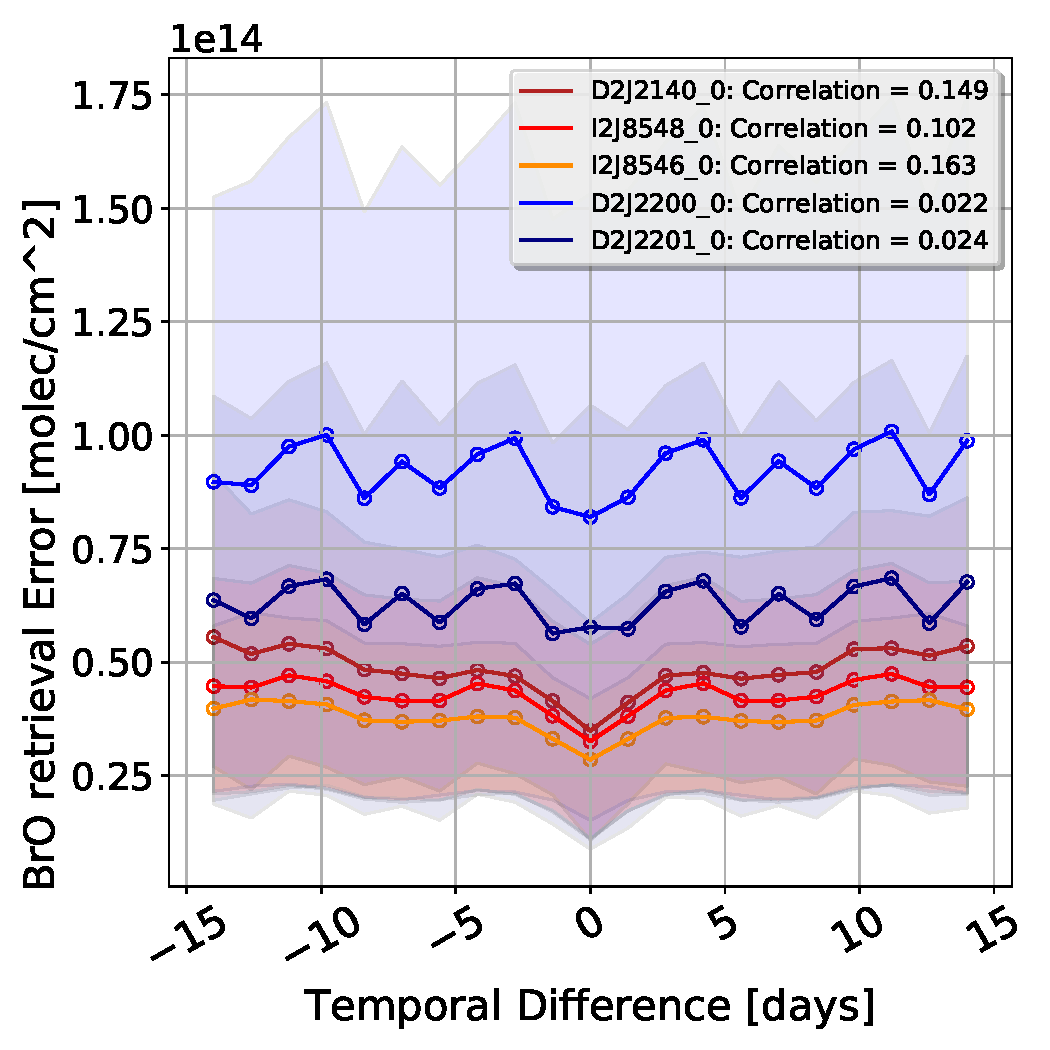
\includegraphics[width=0.7\linewidth]{Bilder/DatallInstruments}
	\caption{The \ce{BrO} measurement error as a function of the temporal difference in days between the reference and the plume is shown for each of the individual instruments at Tungurahua and Nevado del Ruiz. The instruments at Nevado del Ruiz are coloured in blue, while the instruments at Tungurahua are coloured in red colour tones.  To evaluate the plume spectra all reference spectra with a temporal distance of no longer than two weeks are used. An increase of the \ce{BrO} error with the absolute difference in temperature is observable. This is quantified by a correlation between the \ce{BrO} retrieval error and the absolute temporal difference. The plots reveal a symmetry around the axis with zero temperature difference.}
	\label{fig:datallinstruments}
\end{figure}
%
\Cref{fig:dat} (b) shows the evolution of the \ce{BrO} error for a maximal absolute temporal difference of 120 hours. It is only possible to record data during daytime. This causes the lack of data in the night time. A periodic decrease of the \ce{BrO} error can be seen. This is a result of a decrease of the \ce{BrO} error when the ambient conditions coincidence. In this case the daytime coincidence causes the \ce{BrO}  error decrease. This effect is analysed in detail in the following.


\subsection{ Daytime \label{chap:daytime}}
\begin{figure}
	\centering
	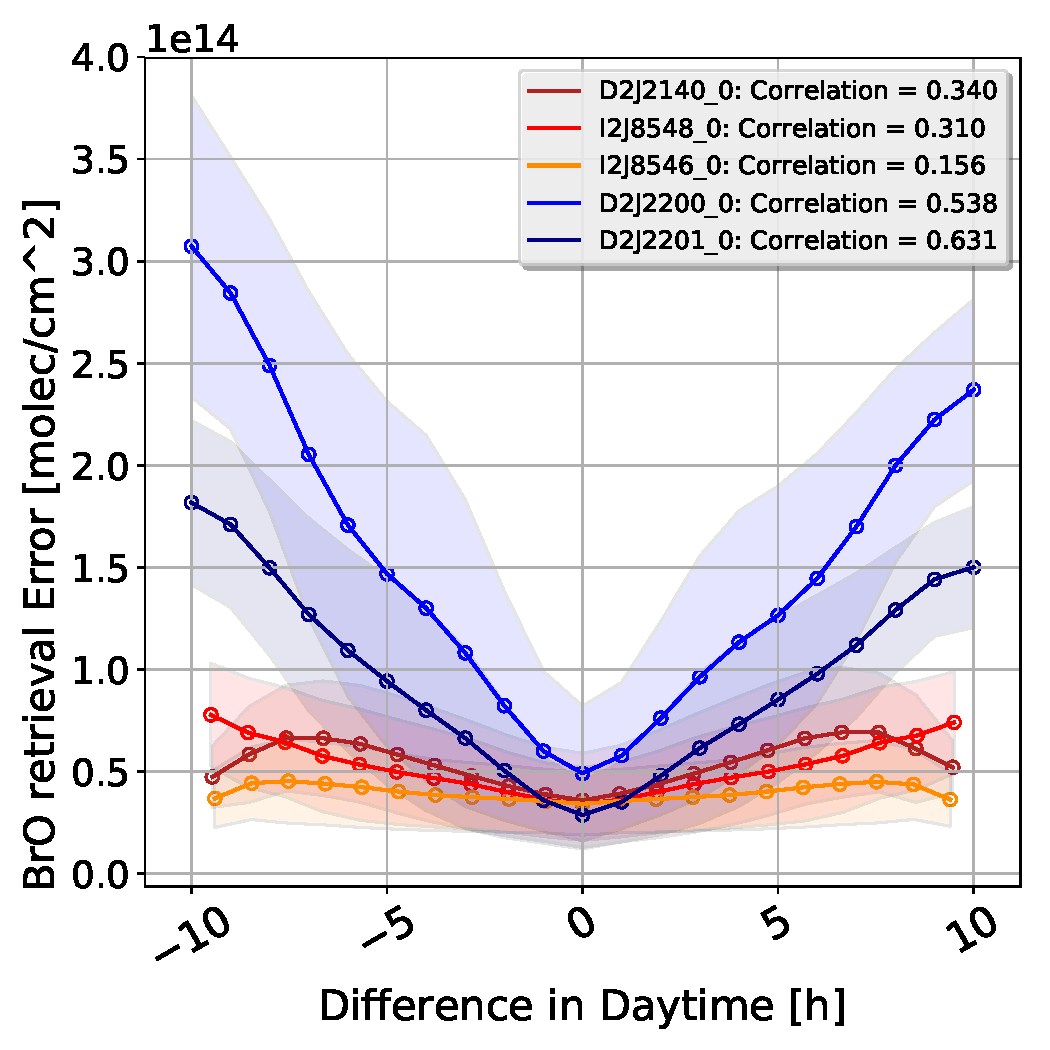
\includegraphics[width=0.7\linewidth]{Bilder/DiffDaytimeallInstruments}
	\caption{The \ce{BrO} measurement error as a function of the difference of daytime between the reference and the plume is shown for each of the individual instruments at Tungurahua and Nevado del Ruiz. To evaluate the plume spectra all reference spectra with a temporal distance of no longer than two weeks are used. An increase of the \ce{BrO} error with the absolute difference in daytime is observable. This is quantified by a correlation between the \ce{BrO} retrieval error and the absolute difference in daytime. The plots reveal a symmetry around axis with zero daytime difference. }
	\label{fig:diffdaytime}
\end{figure}
% individual text
Here I discuss the dependency of the BrO retrieval error based on the bulk effect of a difference in daytime. During the day a lot of external parameters like temperature, solar zenith angle etc. change. In particular, the solar zenith angle could have an impact on the fit quality since the light path of the sun is much longer in the morning or evening compared to the noon. Therefore, the scattering effects and the light intensity are different for both spectra.\\

% fig_curves
In \cref{fig:diffdaytime} the \ce{BrO} error is plotted against the daytime difference between the plume spectrum and the reference spectrum.  \\
Because of the observed symmetry around zero the absolute daytime difference is used for the fit. The computed fitting parameters slope and intercept for each instrument are shown in tab. \ref{tab:dtcalc}. \\
%
As it can be seen in tab. \ref{tab:dtcalc}, the intercepts, which defines the main BrO retrieval error for a daytime difference of zero, vary at Tungurahua between 3.28$\cdot10^{13}\frac{molec}{cm^2}$ and 3.43$\cdot10^{13}\frac{molec}{cm^2}$. The variation at Nevado del Ruiz ranges from  2.24$\cdot10^{13}\frac{molec}{cm^2}$ to 4.01$\cdot10^{13}\frac{molec}{cm^2}$. \\
The correlation coefficient between daytime und BrO fit error 
ranges from 0.156 for the instrument I2J8546 to  0.631 for D2J2201 and exhibits a large variation between the instruments. This lead to the conclusion, that the dependence of the fit quality on the daytime depends largely on the location of the instrument.\\
The $\Delta DT_{2}$, the daytime difference for which the BrO retrieval error doubles compared to a daytime difference of zero is rather high for the instruments installed at Tungurahua (6.8h to 24.2h) and rather low for the instruments installed at Nevado del Ruiz (11.62h to 1.9h).

% tab_fit CAPTION
\begin{table}[h]
	\centering	
	\caption{The \ce{BrO} measurement error as a function of the difference of daytime in hours between the reference and the plume is fitted with a first order polynomial for each of the individual instruments at Tungurahua and Nevado del Ruiz. This table shows the fitting parameters slope and intercept. Moreover, the correlation between the \ce{BrO} error and the absolute daytime difference is shown. In the $\Delta DT_{2}$ row the daytime difference for which the error doubles compared to a daytime difference of zero is shown.}
	\fbox{\begin{tabular}{p{2cm}p{2.15cm}p{2.15cm}p{2.15cm}p{2.15cm}p{2.15cm}}
		%	\toprule
		Instrument	&D2J2140&I2J8546& I2J8548&D2J2200&D2J2201\\
		\toprule
		Slope&5.07$\cdot10^{12}$&1.40$\cdot10^{12}$ &3.77$\cdot10^{12}$&2.04$\cdot10^{13}$& 1.38$\cdot 10^{13}$\\
	%	%midrule
		Correlation&
		0.340&
		0.156&
		0.310&
		0.538&
		0.631\\
	%	%midrule
		Intercept& 3.43$\cdot10^{13}$&3.39$\cdot10^{13}$&3.28$\cdot10^{13}$&  4.01$\cdot10^{13}$&  2.24$\cdot10^{13}$\\
	%	%midrule
		$\Delta DT_{2}$&6.8&24.2&8.7&1.9&1.62\\
	%	%\bottomrule
	\end{tabular}}
	\label{tab:dtcalc}

\end{table}

% tab_ratio CAPTION
\begin{table}
	\centering	
	\caption{This table shows the absolute amount and the percentage corresponding to initial number of references without any restrictions of ambient conditions (table 6.1) of remaining references if restricting the daytime difference to the mean $\Delta DT_{2}$ over all instruments except I2J8546 due to the large uncertainty ($Mean(\Delta DT_{2}) = 4.75h$). Here in the ”Mean” and “Std” row for each  instrument the average restriction is shown with the corresponding standard deviation. The “Min” and “Max” rows show the extend of restriction in the extreme cases (minimum and maximum amount of available references / restriction ratio).}
	\fbox{\begin{tabular}{p{1.8cm}p{2.15cm}p{2.15cm}p{2.15cm}p{2.15cm}p{2.15cm}}
		%	\toprule
		Instrument	&D2J2140&I2J8546& I2J8548&D2J2200&D2J2201\\
		\toprule
		Mean&
		72.0 ($\entspricht\,$85.1\%) &		147.4 ($\entspricht\,$90.0\%)&
		198.4 ($\entspricht\,$91.4\%)&		275.0 ($\entspricht\,$96.8\%)&
		205.8 ($\entspricht\,$91.2\%)\\
		%midrule
		\myrowcolour%
		Std&		31.87 ($\entspricht\,$89.0\%)&32.0 ($\entspricht\,$107.0\%)&
		71.0 ($\entspricht\,$109.5\%)&		70.8 ($\entspricht\,$101.8\%)&
		50.1 ($\entspricht\,$121.6\%) \\
		%midrule
		Min&
		6 $\qquad$($\entspricht\,$75.0\%)&		58 ($\entspricht\,$51.3\%)
		&91 ($\entspricht\,$93.8\%)		&54 ($\entspricht\,$84.4\%)
		&45 ($\entspricht\,$71.4\%)\\
		%midrule
		\myrowcolour%
		Max&
		160 ($\entspricht\,$94.7\%) &
		214 ($\entspricht\,$100\%) &
		399 ($\entspricht\,$100\%) &
		433 ($\entspricht\,$100\%) &
		297 ($\entspricht\,$100\%) \\
		%\bottomrule
	\end{tabular}}

	\label{tab:daytimerest}
\end{table}	
% tab_ratio
The mean ($Mean(\Delta DT_{2})$) is calculated without taking the instrument I2J8546 into account due to the low correlation of 0.156. Using the I2J8546 instrument as well would lead to an  $Mean(\Delta DT_{2})$ of $8.6h$, thus, the restriction would not have any influence, since the maximal time difference is limited to the time where the sun is shining.\\ 
Excluding references with daytime differences above $4.75$h restricts the amount of potential references to $85.1\%$ for D2J2140 to $96.8\%$ for D2J2200. In extreme cases a restriction down to $51.3\%$ of the entire set of references can occur (see \cref{tab:daytimerest}).



\subsection{Temperature}
% fig_curves CAPTION
\begin{figure}
	\centering
	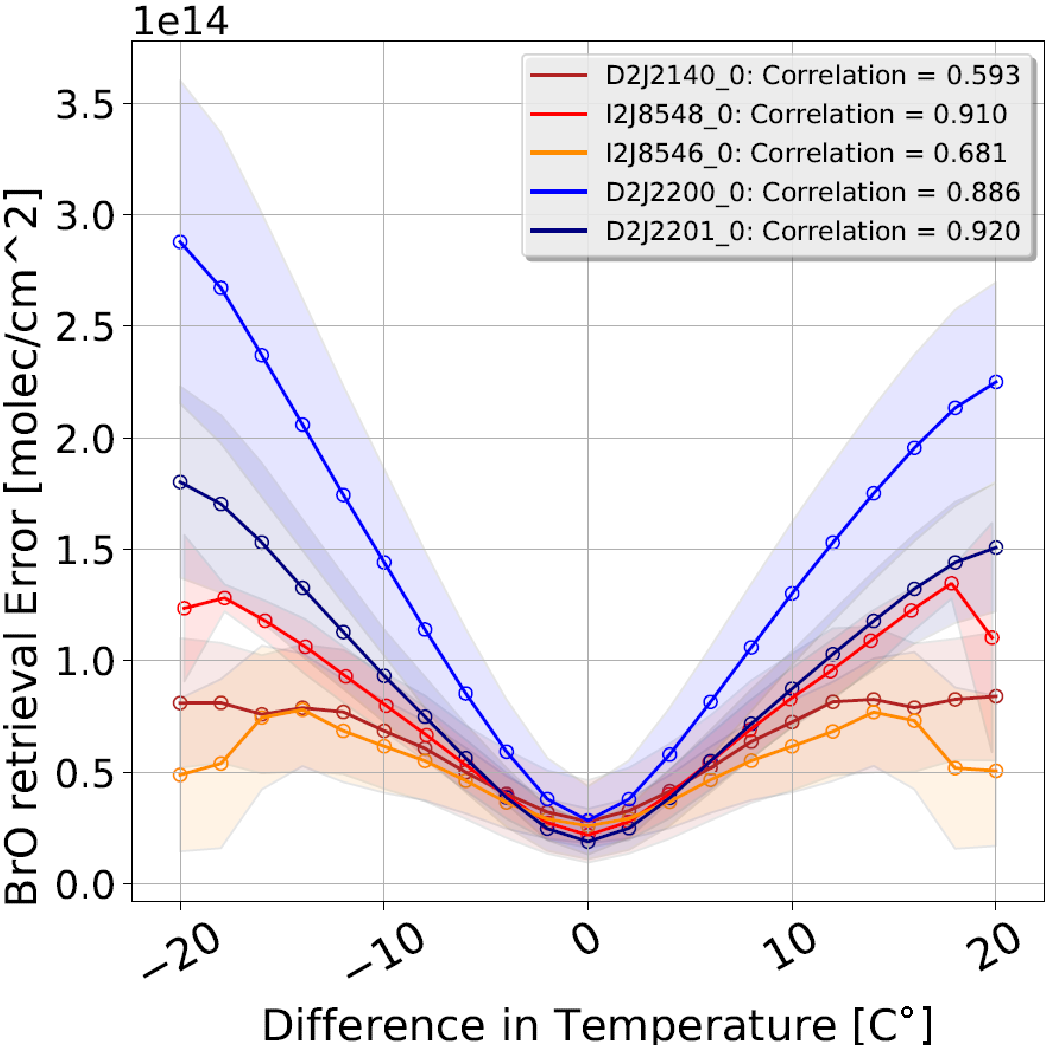
\includegraphics[width=0.7\linewidth]{Bilder/DiffTempallInstruments1}
	\caption{The \ce{BrO} measurement error as a function of the difference of temperature between the reference and the plume is shown for each of the individual instruments at Tungurahua and Nevado del Ruiz. To evaluate the plume spectra all reference spectra with a temporal distance of no longer than two weeks are used. An increase of the \ce{BrO} error with the absolute difference in temperature is observable. This is quantified by a correlation between the \ce{BrO} retrieval error and the absolute difference in temperature. The plots reveal a symmetry around the axis with zero temperature difference.}
	\label{fig:difftemp}
\end{figure}
% individual text
In this section I discuss the particular effect of a difference in temperature, which has been shown to be the most important influence.
The instrument design of the NOVAC instruments compromises between accuracy and robustness as explained in \cref{NOVAC}. In particular, there are no internal thermal stabilizations installed as an attempt to reduce the instruments power consumption and increase the robustness. This can influence the recorded spectra.\\
The ambient temperature however has an influence on the optical adjustment of the NOVAC instrument and thus on the instrument line function and calibration of the spectrometer.
The calibration for the wavelength to pixel mapping (WPM) is commonly determined by a mercury lamp or by the comparison with the high defined Kuruz spectrum.
As the WPM depends on the optical alignment of the spectrometer, which itself depends on the temperature, it is not constant.
Changes in the spectrometers temperature can cause changes in the instrument line function and shifts in the WPM (\citep{pinardi2007influence}). 
% short term wavelength
\begin{figure}		
	\subfigure[]{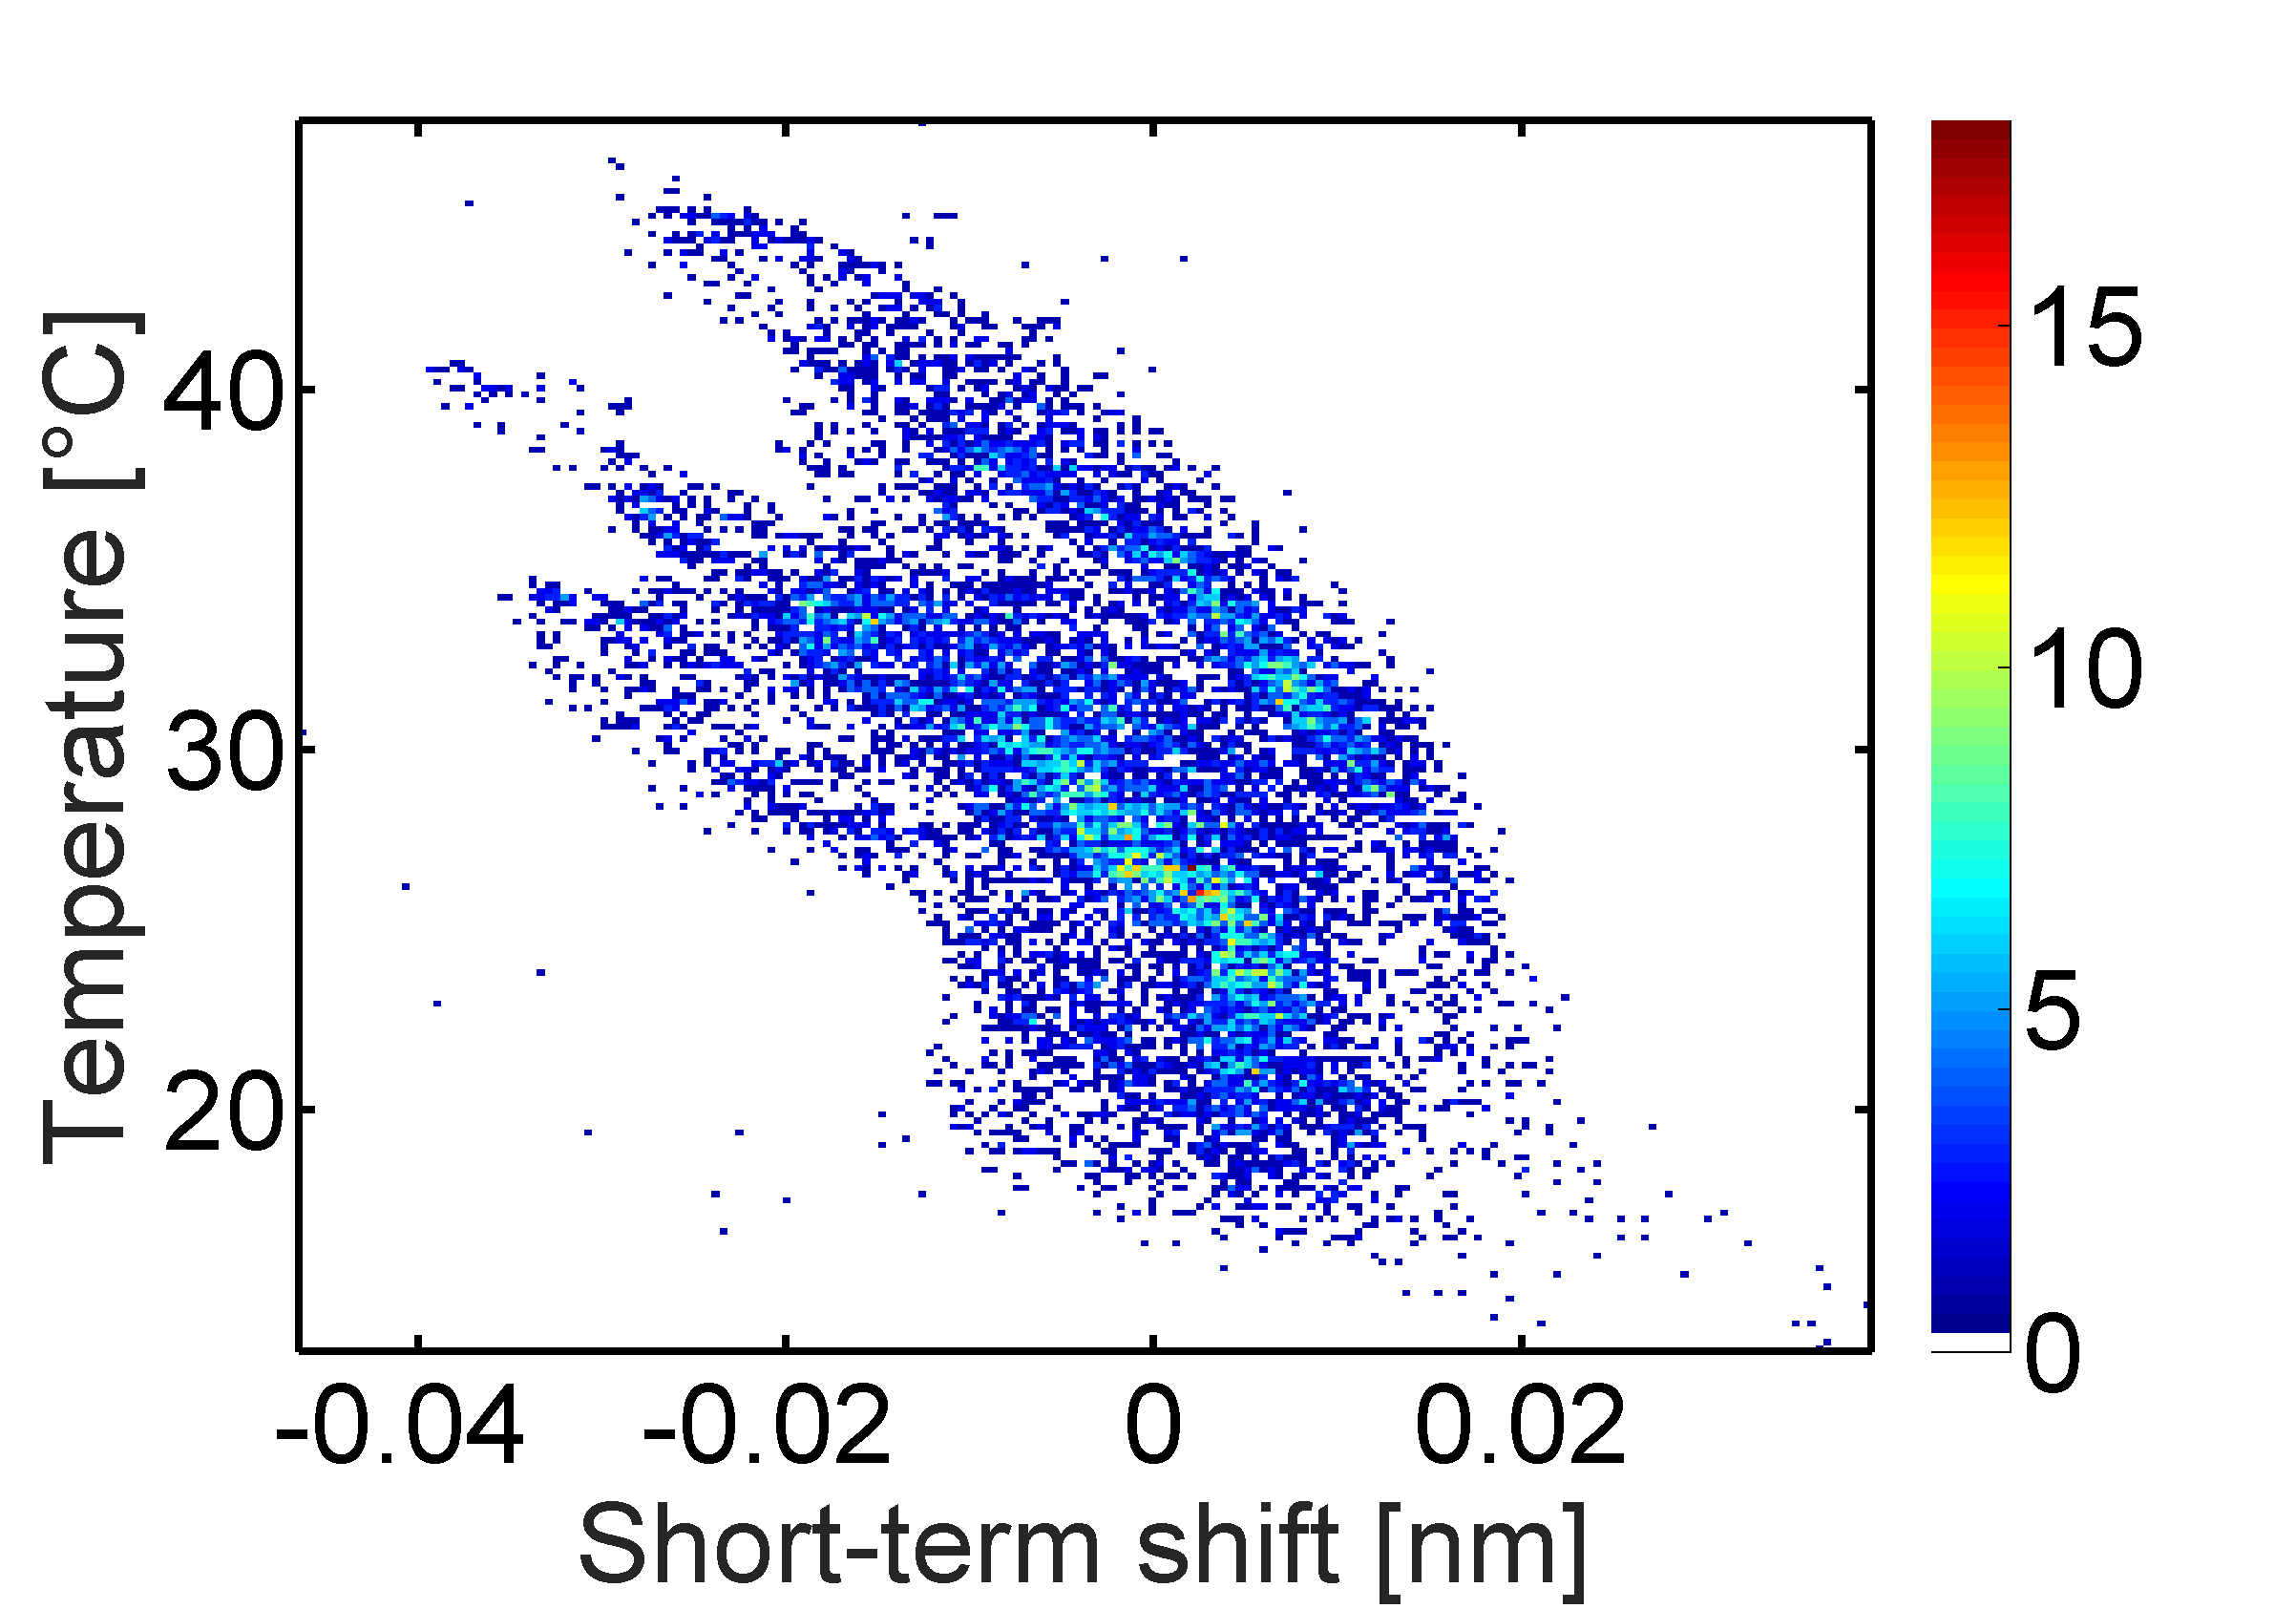
\includegraphics[width=0.49\textwidth]{Bilder/Simon/Bilder_Tung/D2J2140_Before}}
	\subfigure[]{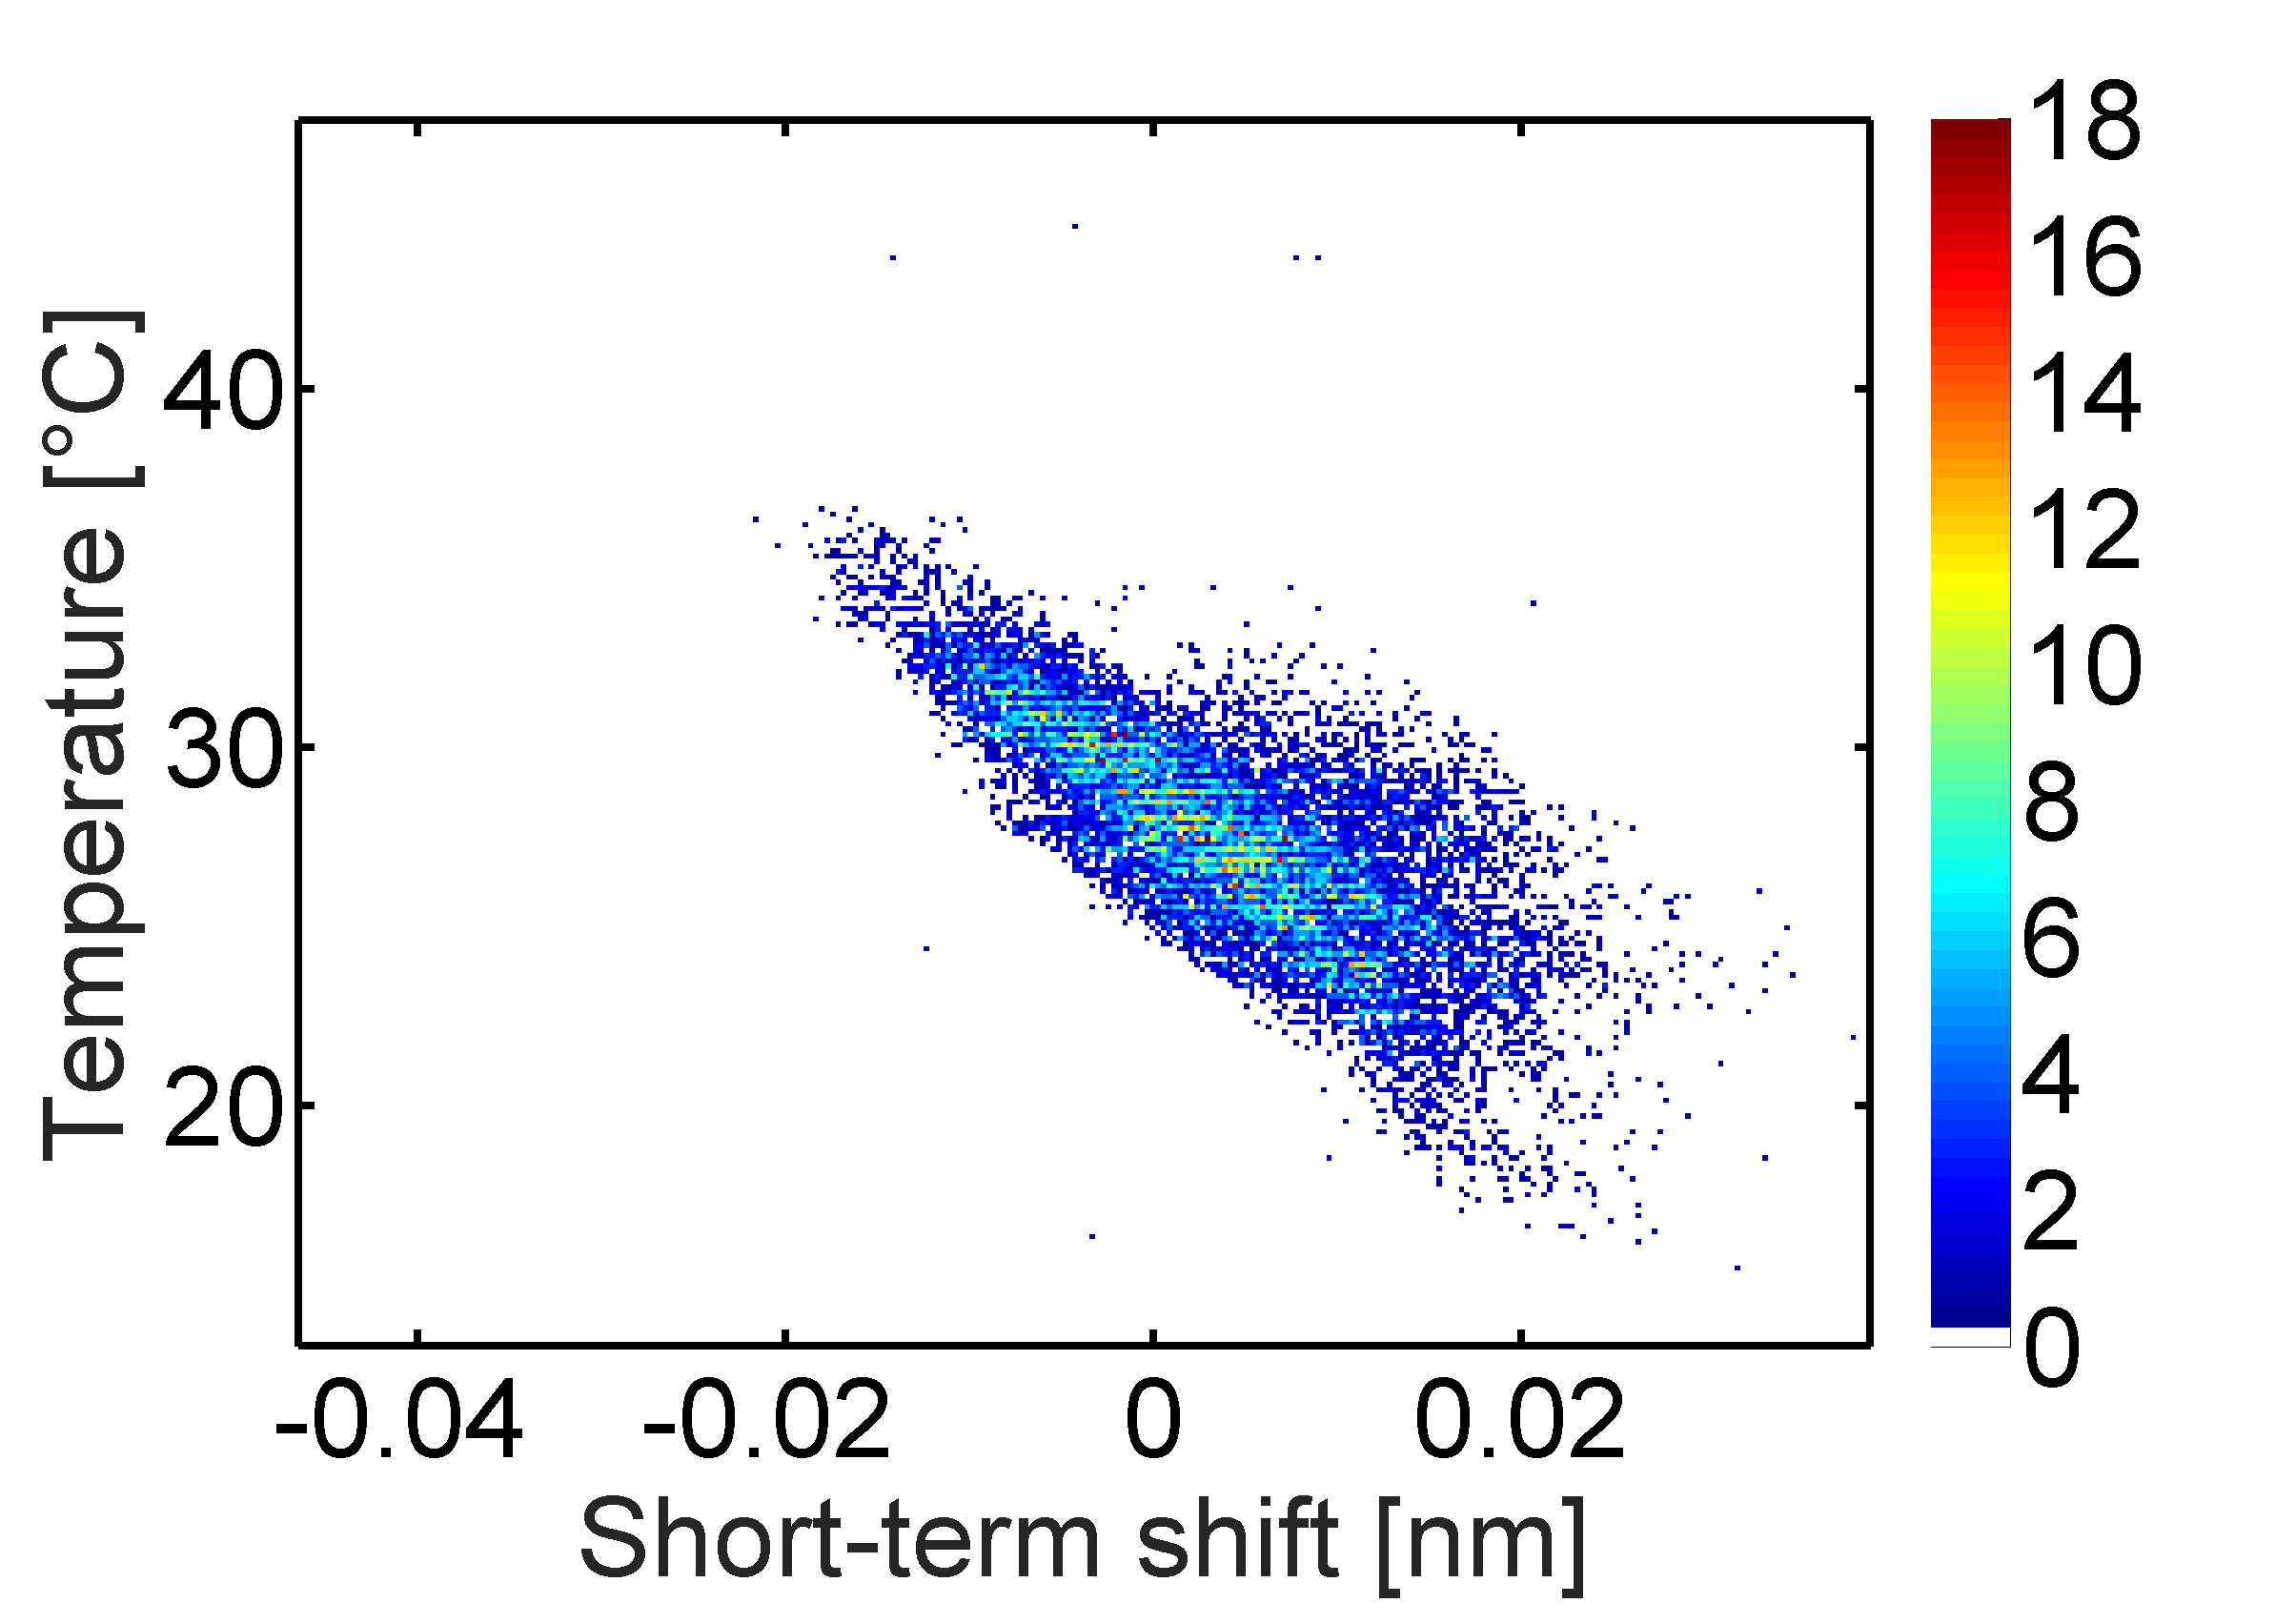
\includegraphics[width=0.49\textwidth]{Bilder/Simon/Bilder_Tung/D2J2140_After}}
	\caption{Short term wavelength as a function of the instrument temperature for Pillate 1. The coloring of the scatter points indicate the temporal evolvement. (a) initial period prior to January 2010 (b) after 2010. Source: \cite{WarnachSimon}.}
	\label{fig:shorttermshift}
\end{figure}
Moreover, \cite{WarnachSimon} show that, short term shifts are related to the instrument temperature (see \cref{fig:shorttermshift}).\\
The above discussed temperature dependence of the instrument line function causes a reduction of the fit quality with increasing instrument temperature difference between plume and reference (see \cref{fig:difftemp}). Thus, the \ce{BrO} error also increases with the temperature difference.
Compared to the other external parameters the temperature difference has the largest impact on the \ce{BrO} error.\\
\\
% tab_fit CAPTION
\begin{table}[h]
	\centering	
	\caption{The \ce{BrO} measurement error as a function of the difference of temperature between the reference and the plume is fitted with a first order polynomial for each of the individual instruments at Tungurahua and Nevado del Ruiz. This table shows the fitting parameters slope and intercept. Moreover, the correlation between the \ce{BrO} error and the absolute temperature difference is shown. For the temperature difference this correlation with an average of $0.797$ is the highest compared to the other external parameters. In the $\Delta T_{2}$ row the temperature difference for which the error doubles compared to a temperature difference of zero is shown. This is already the case for a difference of $3.3^\circ C$}
	\fbox{\begin{tabular}{p{2cm}p{2cm}p{2cm}p{2cm}p{2cm}p{2cm}}
		%	\toprule
		Instrument	&D2J2140&I2J8546& I2J8548&D2J2200&D2J2201\\
		\toprule
		Slope&4.10$\cdot10^{12}$ &3.93$\cdot10^{12}$ &6.50$\cdot10^{12}$ &1.24$\cdot10^{13}$&8.17$\cdot10^{12}$ \\
		%midrule
		Correlation
		& 
		0.593& 
		0.681& 
		0.910& 
		0.886& 
		0.920\\
		%midrule
		Intercept&2.58$\cdot10^{13}$&2.23$\cdot10^{13}$&1.60$\cdot10^{13}$& 1.38$\cdot10^{13}$& 9.07$\cdot10^{12}$\\
		%midrule
		$\Delta T_{2}$&6.3&5.7&2.5&1.1&1.1\\
		%\bottomrule
	\end{tabular}}
	\label{tab:tempe}

\end{table}
% tab_fit
% fig_curves
The plots reveal a symmetry around axis with zero temperature difference (see \cref{fig:difftemp}), thus using only the absolute temperature difference for the fit is reasonable.\\
The intercepts for the BrO fit error at Tungurahua vary from 1.6$\cdot10^{13}\frac{molec}{cm^2}$ to 2.58$\cdot10^{13}\frac{molec}{cm^2}$ (see tab. \ref{tab:tempe}). The intercepts at Nevado del Ruiz are lower and ranges from  9.07$\cdot10^{12}\frac{molec}{cm^2}$ to 1.38$\cdot10^{13}\frac{molec}{cm^2}$. The $\Delta T_{2}$ from the data of Tungurahua (2.5 K to 6.3K) are significantly higher as at Nevado del Ruiz (1.1 K). The mean $\Delta T_{2}$ is $ 3.3$K. The conclusion is, that the temperature has a stronger influence at the Nevado del Ruiz volcano.\\
The correlation between the \ce{BrO} error and the absolute temperature difference has a high significance. 
The correlation coefficients ranges from 0.593 for the instrument D2J2140 to  0.92 for D2J2201 and exhibits a large variation between the instruments. \\
The computed fitting parameters slope and intercept for each instrument are shown in tab. \ref{tab:tempe}.\\
% tab_ratio CAPTION
\begin{table}
	\centering	
	\caption{This table shows the absolute amount and the ratio (to \cref{Tab:refstime}) of remaining references if restricting the temperature difference to the mean $\Delta T_{2}$ over all instruments ($Mean(\Delta T_{2}) = 3.3^{\circ}C$). Here in the ”Mean” and “Std” row for each  instrument the average restriction is shown with the corresponding standard deviation. The “Min” and “Max” rows show the extend of restriction in the extreme cases (minimum and maximum amount of available references / restriction ratio).}
	\fbox{\begin{tabular}{p{1.8cm}p{2.15cm}p{2.15cm}p{2.15cm}p{2.15cm}p{2.15cm}}
		%	\toprule
		Instrument	&D2J2140&I2J8546& I2J8548&D2J2200&D2J2201\\
		\toprule
		Mean&
		39.6 ($\entspricht\,$46.8\%)&
		119.3 ($\entspricht\,$72.9\%)
		&158.2 ($\entspricht\,$72.9\%)
		&233.6 ($\entspricht\,$82.3\%)
		&151.6 ($\entspricht\,$67.2\%)\\
		%midrule
		\myrowcolour%
		Std&
		24.7 ($\entspricht\,$68.9\%)&
		50.4 ($\entspricht\,$168.6\%)&
		76.0 ($\entspricht\,$117.2\%)&
		84.5 ($\entspricht\,$121.6\%)&
		72.6 ($\entspricht\,$176.2\%)\\
		%midrule
		Min&
		1 ($\entspricht\,$12.5\%)
		&8 ($\entspricht\,$7.1\%)&
		12 ($\entspricht\,$12.4\%)&
		3 ($\entspricht\,$4.7\%) &
		6 ($\entspricht\,$9.5\%)\\
		%midrule
		\myrowcolour
		Max
		&
		130	 ($\entspricht\,$76.9\%)&
		213	 ($\entspricht\,$99.5\%)&
		386 ($\entspricht\,$96.7\%)&
		414	 ($\entspricht\,$95.6\%) &
		296	 ($\entspricht\,$99.7\%)\\
		%\bottomrule
	\end{tabular}}

	\label{tab:decTemp}
\end{table}	
% tab_ratio
If restricting the temperature difference to the mean $\Delta T_{2}$ over all instruments ($Mean(\Delta T_{2}) = 3.3$) the amount of possible references decrease as shown in tab. \ref{tab:decTemp}. Excluding references with temperature differences above $Mean(\Delta T_{2}) = 3.3$ restricts the amount of potential references to $46.8\%$ for the $D2J2140$ instrument to $82.3\%$ for the $D2J2200$ instrument.

\subsection{ Colour index}
\begin{figure}
	\centering
	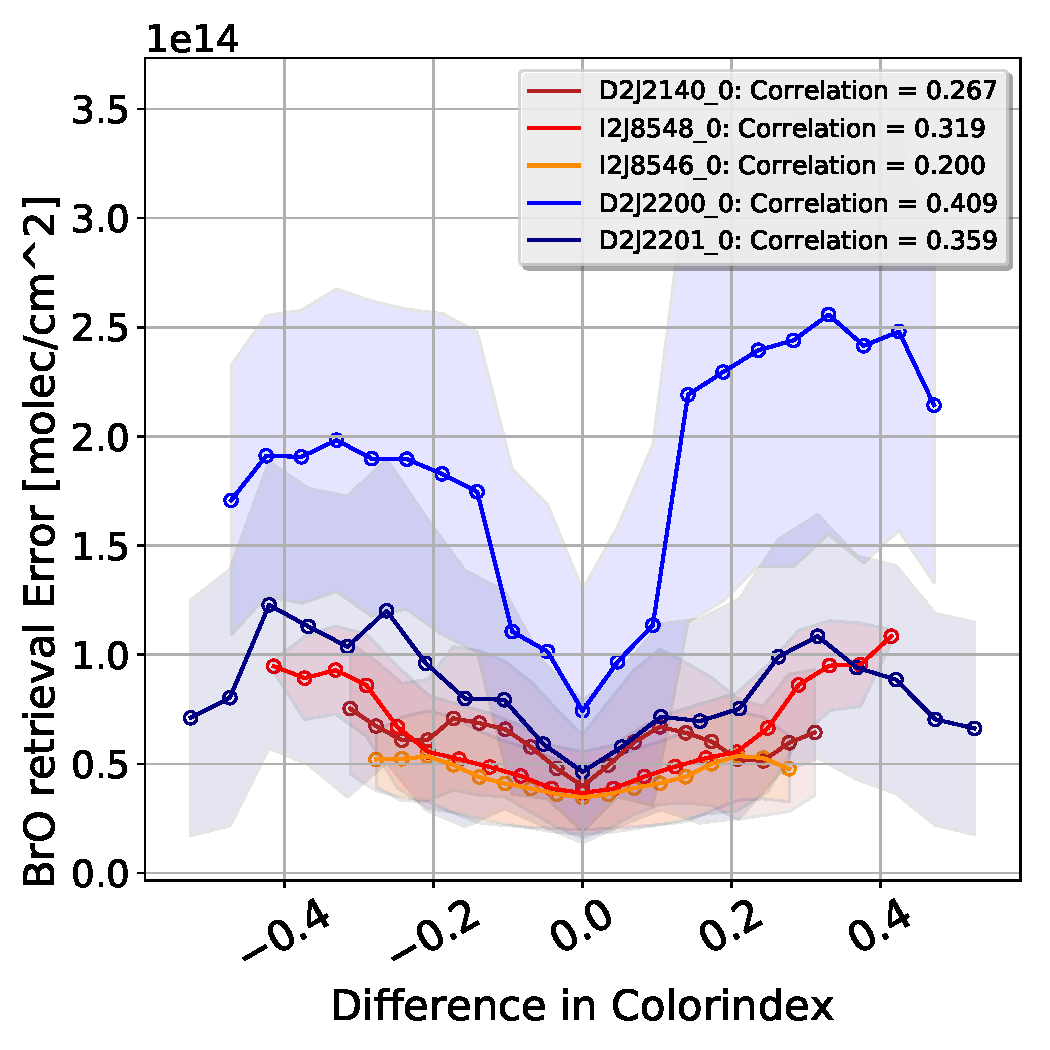
\includegraphics[width=0.7\linewidth]{Bilder/DiffColidxallInstruments}
	\caption{The \ce{BrO} measurement error as a function of the difference of colour index between the reference and the plume is shown for each of the individual instruments at Tungurahua and Nevado del Ruiz. To evaluate the plume spectra all reference spectra with a temporal distance of no longer than two weeks are used. An increase of the \ce{BrO} error with the absolute difference in colour index is observable. This is quantified by a correlation between the \ce{BrO} retrieval error and the absolute difference in colour index. The plots reveal a symmetry around axis with zero colour index difference. }
	\label{fig:diffcolidx}
\end{figure}
% individual text
Clouds  have  a  strong  influence  on  the  atmospheric  radiative  transfer  and  thus  affect  the  interpretation  and  analysis of DOAS \citep{wagner2014cloud}.
Clouds can be identified by several measurement quantities which they influence.
As Mie scattering is dominant in clouds the wavelength dependency of the light that is scattered is different than the Rayleigh sky. Thus, clouds can be easily identified by their white color.
Therefore, the cloudiness of the sky can be quantified in a scalar measure defined by the ratio of the measured intensity at two wavelengths, the so-called colour index.
\cite{wagner2014cloud} showed that for a zenith-looking instrument the measured radiation intensity is enhanced by clouds. Thus, clouds can cause large errors for the retrieved gas column density and the corresponding uncertainties. 
Cloud effects are especially severe if the cloudiness for the recorded plume and reference spectra strongly defer. Also for broken clouds the described effect can be observed as measurements at some elevation angles might be influenced by clouds while others are not.
In this work I use the Colour Index (CI) between the intensities at 320nm and 360 nm.
These two wavelengths are as far apart as the filter used for stray-light prevention in the spectrometers allows.
%% I don’t understand 	
On the other hand, the lower wavelength avoids the deep UV range where \ce{SO2} and  \ce{O3} absorption plays a dominant role.
%% I don’t understand 	
The Mie scattering in the clouds is responsible for the higher amount of radiation from larger wavelengths. This results in a decrease of the CI which was observed for NOVAC instruments by \citet{lubcke2014optical}.\\
I evaluated the CI at the zenith. To increase the stability of the fit I add 10 the intensities from 10 consecutive spectra. Using always the zenith to evaluate the colour index makes the colour index more comparable, but if broken clouds occur, the CI of the reference and the plume could differ from the calculated CI of the zenith. This could be a reason for the large deviations of the mean \ce{BrO} error as function of the colour index (see \cref{fig:diffcolidx})\\
% fig_curves
In \cref{fig:diffcolidx} the \ce{BrO} error is plotted against the colour index difference between the plume and the reference spectrum. The plot is done similar as the plots for the temperature.
The plots mostly reveal a symmetry around the zero colour index difference-axis. Thus, the absolute colour index can be used for the fitting which is done equivalently to the analysis of the temperature and the daytime. The computed fitting parameters slope and intercept for each instrument are shown in \cref{tab:colidxcalc}. \\
The intercepts at Tungurahua vary from 3.36$\cdot10^{13}\frac{molec}{cm^2}$ to 4.01$\cdot10^{13}\frac{molec}{cm^2}$. The variation at Nevado del Ruiz ranges from  4.74$\cdot10^{13}\frac{molec}{cm^2}$ to 7.21$\cdot10^{13}\frac{molec}{cm^2}$.\\
The correlation is as well calculated and ranges from 0.2 for the instrument I2J8546 to  0.409 for D2J2200.\\
\begin{table}[h]
	\centering	
	\caption{The \ce{BrO} measurement error as a function of the difference of colour index between the reference and the plume is fitted with a first order polynomial for each of the individual instruments at Tungurahua and Nevado del Ruiz. This table shows the fitting parameters slope and intercept. Moreover, the correlation between the \ce{BrO} error and the absolute colour index difference is shown. In the $\Delta CI_{2}$ row the colour index difference for which the error doubles compared to a colour index difference of zero is shown.}
	\fbox{\begin{tabular}{p{2cm}p{2cm}p{2cm}p{2cm}p{2cm}p{2cm}}
		%	\toprule
		Instrument	&D2J2140&I2J8546& I2J8548&D2J2200&D2J2201\\
		\toprule
		Slope&2.30$\cdot10^{4}$ &7.92$\cdot10^{13}$ &1.17$\cdot10^{14}$ &5.42$\cdot10^{14}$&1.91$\cdot10^{14}$\\
		%midrule
		Correlation&
		0.267&
		0.200&
		0.319&
		0.409&
		0.359\\
		%midrule
		Intercept&4.01$\cdot10^{13}$&3.36$\cdot10^{13}$&3.47$\cdot10^{13}$& 7.21$\cdot10^{13}$& 4.74$\cdot10^{13}$\\
		%midrule
		$\Delta CI_{2}$&0.174&0.424&0.297&0.133&0.248\\
		%\bottomrule
	\end{tabular}}

	\label{tab:colidxcalc}
\end{table}

% tab_fit CAPTION
\begin{table}[h]
	\centering	
	\caption{This table shows the absolute amount and the ratio  (to \cref{Tab:refstime}) of remaining references if restricting the colour index difference to the mean $\Delta CI_{2}$ over all instruments ($Mean(\Delta CI_{2}) = 0.2553.$). Here in the ”Mean” and “Std” row for each  instrument the average restriction is shown with the corresponding standard deviation. The “Min” and “Max” rows show the extend of restriction in the extreme cases (minimum and maximum amount of available references / restriction ratio).}
	\fbox{\begin{tabular}{p{1.8cm}p{2.15cm}p{2.15cm}p{2.15cm}p{2.15cm}p{2.15cm}}
		% 	\toprule
		Instrument	&D2J2140&I2J8546& I2J8548&D2J2200&D2J2201\\
		\toprule
		Mean&
		84.6 ($\entspricht\,$100\%) &	163.7 ($\entspricht\,$100\%)&	215.6 ($\entspricht\,$99.3\%)&
		275.4 ($\entspricht\,$97.0\%) &219.4 ($\entspricht\,$97.3\%) \\
		%midrule
		\myrowcolour
		Std&
		35.8 ($\entspricht\,$100\%) &	29.9 ($\entspricht\,$100\%) &
		65.4 ($\entspricht\,$101\%)&
		67.8 ($\entspricht\,$97.6\%) &
		49.86 ($\entspricht\,$121\%) \\
		%midrule
		Min&
		8 ($\entspricht\,$100\%) &
		113 ($\entspricht\,$100\%) 
		&97 ($\entspricht\,$100\%) 
		&61 ($\entspricht\,$95.3\%) 
		&28	 ($\entspricht\,$44.4\%) \\
		%midrule
		\myrowcolour
		Max
		&169 ($\entspricht\,$100\%) 
		&214 ($\entspricht\,$100\%) 
		&399 ($\entspricht\,$100\%) 
		&421 ($\entspricht\,$97.2\%) 
		&297 ($\entspricht\,$100\%)  \\
		%\bottomrule
	\end{tabular}}

	\label{tab:colidxres}
\end{table}	
% tab_ratio CAPTION
% tab_ratio
The $\Delta( CI_{2})$ vary from 0.174 to 0.424 at Tungurahua and from 0.133 to 0.248 at Nevado del Ruiz, the
the mean can be calculated as: $Mean(\Delta CI_{2}) = 0.255$. Exclusion of all references with a higher difference in the colour index than $ 0.255$ does not chance the amount of references significantly (see \cref{tab:colidxres}).\\

%\begin{table}
%	\centering
%	\fbox{\begin{tabular}{p{1.8cm}p{2.15cm}p{2.15cm}p{2.15cm}p{2.15cm}p{2.15cm}}
%		%	\toprule
%		Instrument	&D2J2140&I2J8546& I2J8548&D2J2200&D2J2201\\
%		\toprule
%		Mean&38.98&113.8&153.2&223.8&149.37\\
%		%midrule
%		Std&
%		24.47&
%		50.6&
%		76.78&
%		82.5&
%		72.41\\
%		%midrule
%		Min&1&8&12&3 &6\\
%		%midrule
%		Max&130&213&386&399 &296\\
%		%\bottomrule
%	\end{tabular}}
%	\caption{Amount of potential references when restricting the external parameters as discussed above. Here the difference in CI is restricted to $0.2553$, the maximal colourindex difference is $3.358^\circ$,\textcolor{red}{besser}}
%\end{table}	

\subsection{Elevation Angle}

% fig_curves CAPTION
\begin{figure}
	\centering
	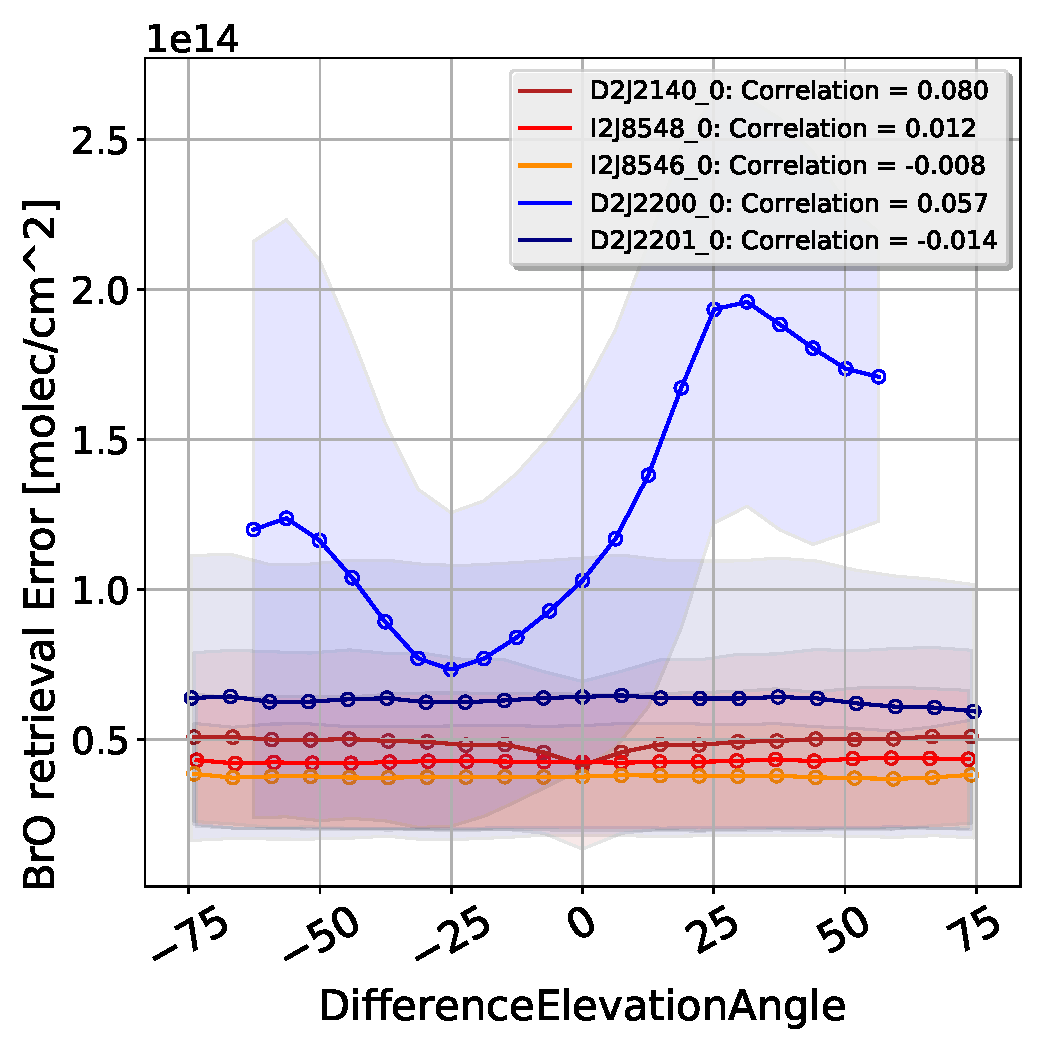
\includegraphics[width=0.7\linewidth]{Bilder/DiffElevAngleallInstruments}
	\caption{The \ce{BrO} measurement error as a function of the difference of elevation angle between the reference and the plume is shown for each of the individual instruments at Tungurahua and Nevado del Ruiz. To evaluate the plume spectra all reference spectra with a temporal distance of no longer than two weeks are used. The plots do not reveal a symmetry around axis with zero elevation angle difference for all instruments. The D2J2200 instrument at Nevado del Ruiz is not symmetric around zero.}
	\label{fig:diffeleangle}
\end{figure}
% tab_fit CAPTION
\begin{table}[h]
	\centering	
	\caption{The \ce{BrO} measurement error as a function of the difference of elevation angle between the reference and the plume is fitted with a first order polynomial for each of the individual instruments at Tungurahua and Nevado del Ruiz. This table shows the fitting parameters slope and intercept. Moreover, the correlation between the \ce{BrO} error and the absolute elevation angle difference is shown. }
	\fbox{\begin{tabular}{p{2cm}p{2cm}p{2cm}p{2cm}p{2cm}p{2cm}}
		%	\toprule
		Instrument	&D2J2140&I2J8546& I2J8548&D2J2200&D2J2201\\
		\toprule
		Slope& 1.73$\cdot10^{8}$& 1.55$\cdot10^{10}$ &-9.00$\cdot10^{9}$ &2.92$\cdot10^{11}$&-3.96$\cdot10^{10}$\\
		%midrule
		Correlation&
		0.000&
		-0.010&
		0.012&
		0.065&
		-0.034\\
		%midrule
		Intercept&4.77$\cdot10^{13}$&4.23$\cdot10^{13}$&3.78$\cdot10^{13}$&8.37$\cdot10^{13}$&6.44$\cdot10^{13}$ \\
		%\bottomrule
	\end{tabular}}

\end{table}
% same daytime / temperature plot 
%\begin{figure}
%	\subfigure{
%		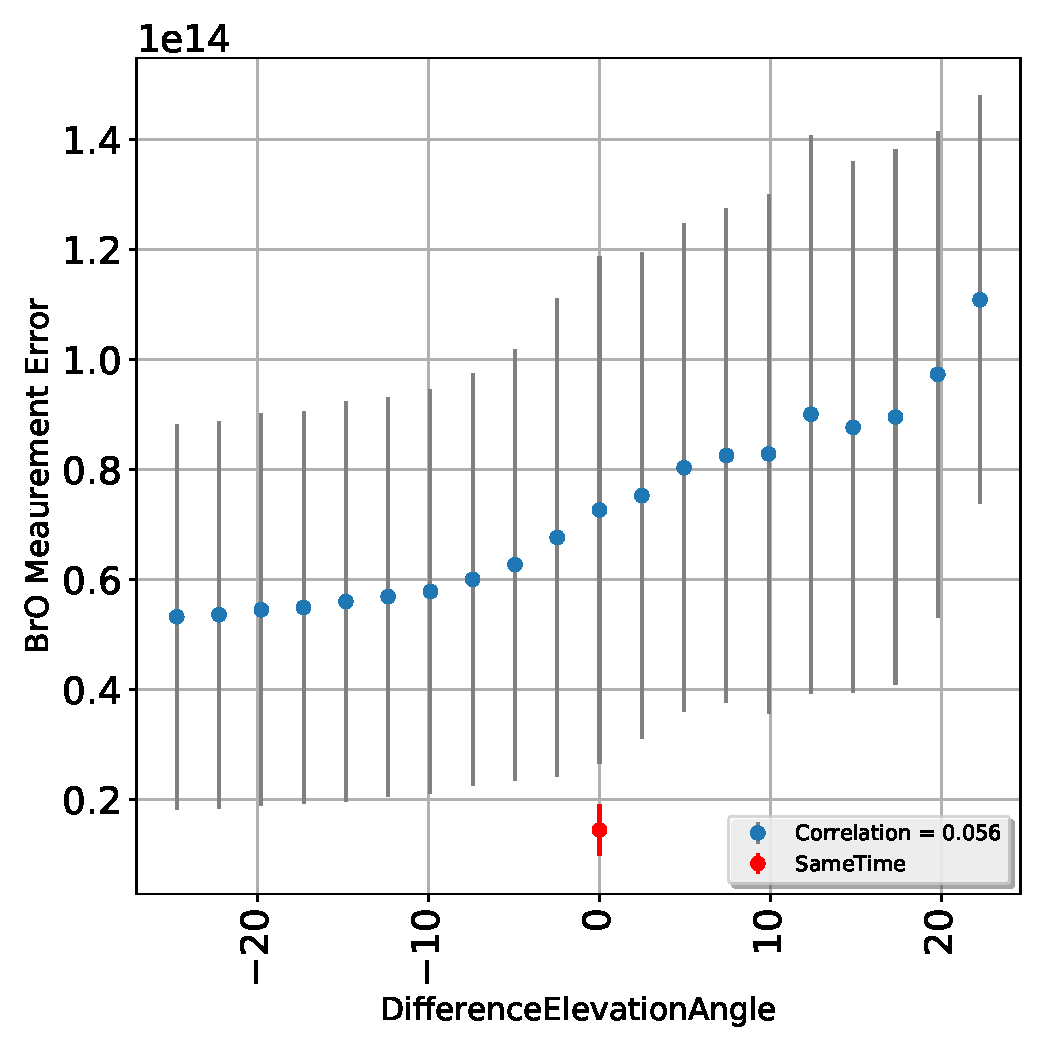
\includegraphics[width=0.49\linewidth]{Bilder/D2J2200_0_DiffElevAngle_onedaytime_Nevad}}
%	\subfigure{
%		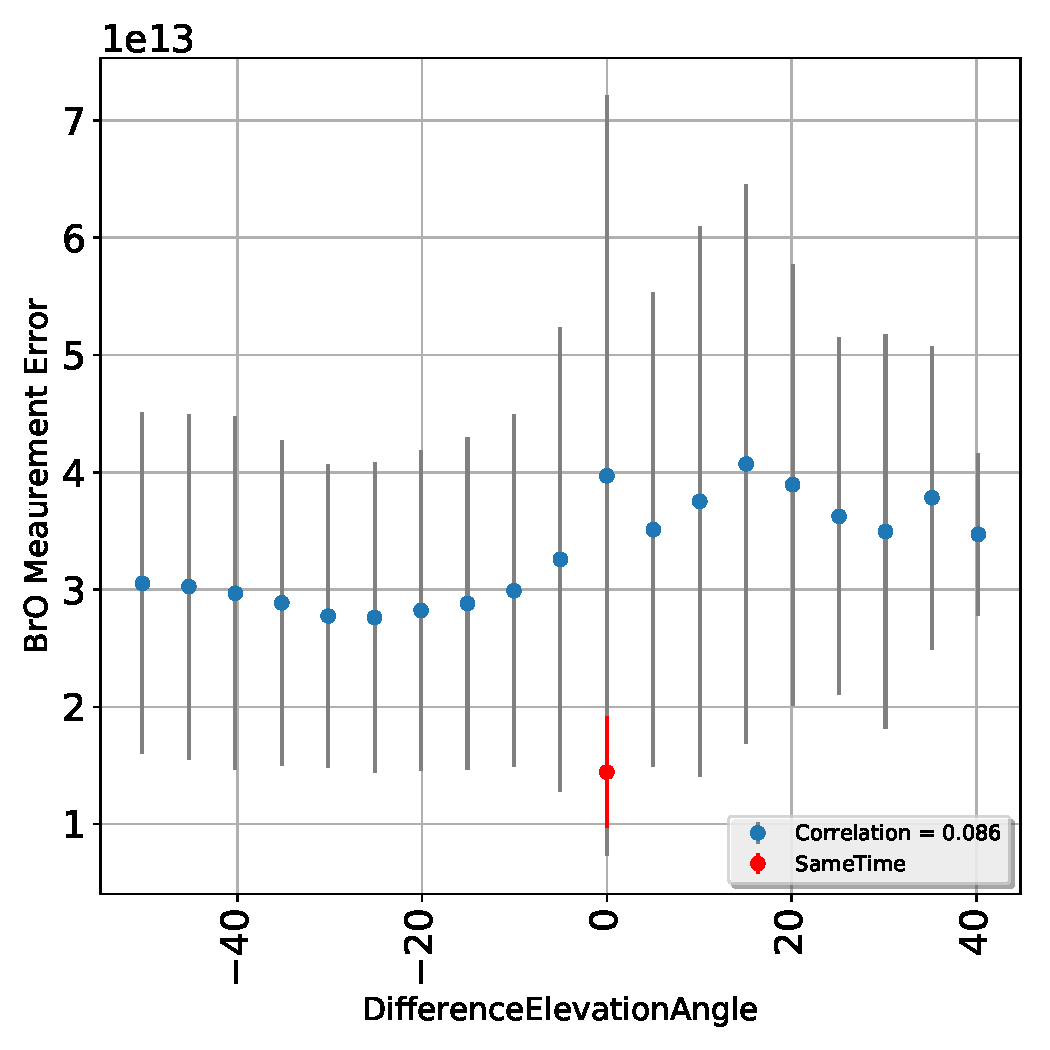
\includegraphics[width=0.49\linewidth]{Bilder/D2J2200_0_DiffElevAngle_onetemp_Nevad}}
%	\caption{The BrO measurement error as a function of the difference of elevation angle between the reference and the plumefor the D2J2200 instrument. Left: restricted to a constant difference in daytime (difference of $\pm 1h$), right: restricted to a constant difference in temperature (difference of $\pm 1^\circ$C).}
%	\label{fig:d2j22000diffelevangleonetempnevad}
%\end{figure}
\begin{figure}
	\centering
	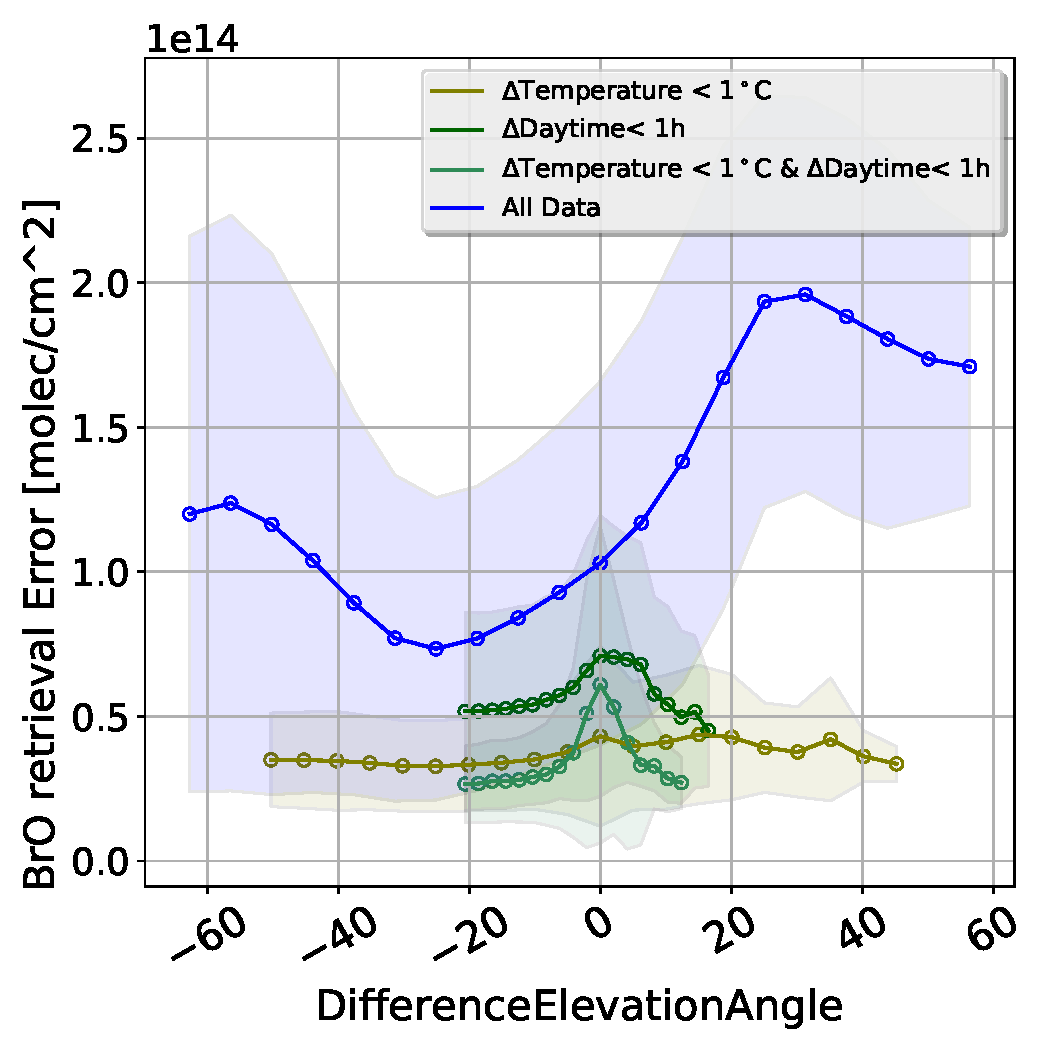
\includegraphics[width=0.7\linewidth]{Bilder/DiffElevAngleKomischesInstr}
	\caption{The \ce{BrO} measurement error as a function of the difference of elevation angle between the reference and the plume for the D2J2200 instrument. To evaluate the origin of the behavior of the \ce{BrO} retrieval error of the D2J2200 instrument as a function of the difference in elevation angle, the data are analysed on its temperature and daytime dependence. The same dependence is shown with restriction to an difference in temperature ($\Delta$Temperature) of below 1$^{\circ}C$ or restriction on a daytime difference of below 1h ($\Delta Daytime \pm 1h$). The curves are marked with different green color tones, as it is shown in the legend. The blue line shows the \ce{BrO} error as function of the elevation angle, when using all data for comprehension.}
	\label{fig:d2j22000diffelevangleonetempnevad}
\end{figure}


The elevation angle describes the angle between the horizon and the zenith. When using the plume spectrum and the reference spectrum of the same time, the difference in elevation angle cannot be zero, since the location of the plume does not coincidence with the location of the reference.\\
In \cref{fig:diffeleangle} the \ce{BrO} error is plotted as a function of the elevation angle. No significant correlation between the two parameters can be identified. \\
Only the data of the D2J2200 instrument significantly vary with the elevation angle. The observable variation of the \ce{BrO} error with the elevation angle differs from the symmetric dependence of all other external parameter, the minimum \ce{BrO} error can be found at a difference in elevation angle of -20$^{\circ}$. This curve is a result of the solar altitude over the day which can be obtained if only using data of the same day time. Such a plot can be seen in \cref{fig:d2j22000diffelevangleonetempnevad}.
\Cref{fig:d2j22000diffelevangleonetempnevad} shows the \ce{BrO} retrieval error as function of the difference elevation angle for the D2J2200 instrument at the Nevado del Ruiz volcano. The blue line is equivalent to the results which are shown in \cref{fig:diffeleangle} for comparison. The green lines show data, with a maximal difference in temperature of 1$^{\circ}C$ or maximal difference in daytime of 1$h$. If restricting the data to just small differences in temperature or/and daytime, the dependency between the \ce{BrO} retrieval and elevation angle appears to be not significant. Whereas the maximum of the \ce{BrO} error can be found at an difference in elevation angle of zero.\\
\\	
Since the \ce{BrO} error does not depend significantly on the elevation angle no restriction on difference of the elevation angle is needed.
\subsection{Exposure time}
\begin{figure}
	\centering
	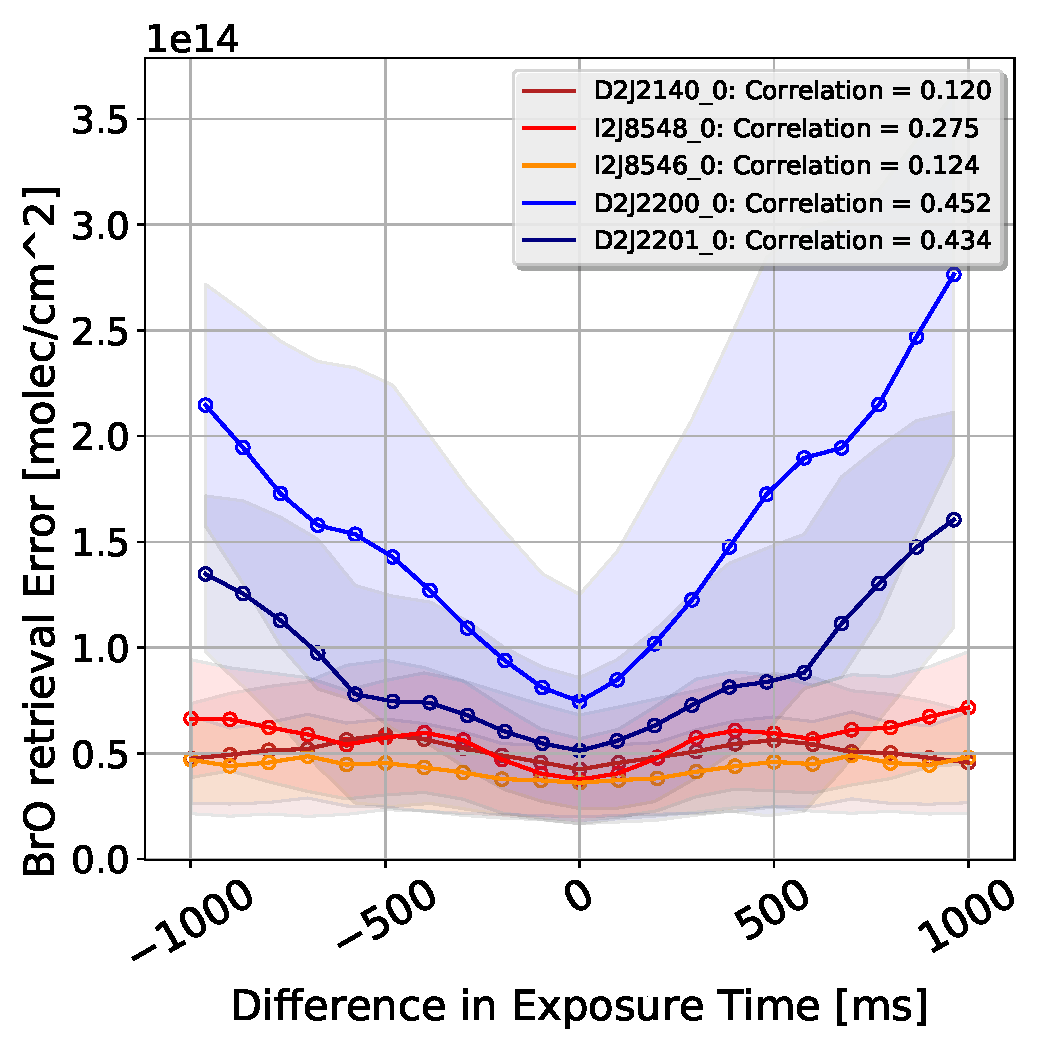
\includegraphics[width=0.7\linewidth]{Bilder/DiffExpTimeallInstruments}
	\caption{The \ce{BrO}  measurement error as a function of the difference of exposure time between measuring the reference and the plume are shown. To evaluate the plume spectra all reference spectra with a temporal distance of no longer than two weeks are used. An increase of the \ce{BrO} error with the distance in exposure time is observable.}
	\label{fig:diffexptime}
\end{figure}
The  exposure time is the length of time the sensor of the NOVAC instrument is exposed to light. In one scan the exposure time is set constant to the exposure time of the first scan, the pre-reference. The amount of light that reaches the film or image sensor is proportional to the exposure time. The exposure time is adjusted in the way that the maximum intensity does not overly the capacity of the sensor. Thus, the exposure time can be used as a proxy for the degree of sky lightness.\\
A small dependency of the \ce{BrO} error on the exposure time can be observed at Tungurahua and Nevado del Ruiz as it is shown in \cref{fig:diffexptime}. The \ce{BrO}  error as a function of the difference in exposure time is also symmetric around zero for all instruments. Thus the absolute difference in the exposure time is sufficient for the evaluation.\\
The instruments at Tungurahua do not show a significant dependence (correlation coefficient between 0.067 and 0.251) on the exposure time, even though there is always a minimum of the \ce{BrO} error at a difference of the Exposure Time of 0ms.\\
Nevado del Ruiz shows a stronger correlation between the \ce{BrO}  error and the exposure time.\\
\begin{table}[h]
	\centering	
	\caption{The \ce{BrO} measurement error as a function of the difference of exposure time between the reference and the plume is fitted with a first order polynomial for each of the individual instruments at Tungurahua and Nevado del Ruiz. This table shows the fitting parameters slope and intercept. Moreover, the correlation between the \ce{BrO} error and the absolute exposure time difference is shown.}
	\fbox{\begin{tabular}{p{2cm}p{2cm}p{2cm}p{2cm}p{2cm}p{2cm}}
		%	\toprule
		Instrument	&D2J2140&I2J8546& I2J8548&D2J2200&D2J2201\\
		\toprule
		Slope& 5.54$\cdot10^{9}$&1.54$\cdot10^{10}$ &3.04$\cdot10^{10}$&1.72$\cdot10^{11}$&9.37$\cdot10^{10}$\\
		%midrule
		Correlation&0.067
		&0.121&
		0.251&
		0.452&
		0.434\\
		%midrule
		Intercept&4.63$\cdot10^{13}$&3.58$\cdot10^{13}$& 3.87$\cdot10^{13}$& 6.88$\cdot10^{13}$& 4.68$\cdot10^{13}$\\
		%midrule
		$\Delta T_{2}$&8357&662&1273&95&499\\
		%\bottomrule
	\end{tabular}}

	\label{tab:exptimecalc}
\end{table}
%
\begin{table}
	\centering	
	\caption{Amount of possible references when restricting the difference in exposure time  between plume and reference to differences below 632.25 ms.}
	\fbox{\begin{tabular}{p{1.8cm}p{2.15cm}p{2.15cm}p{2.15cm}p{2.15cm}p{2.15cm}}
		%	\toprule
		Instrument	&D2J2140&I2J8546& I2J8548&D2J2200&D2J2201\\
		\toprule
		Mean&
		81.7 ($\entspricht\,$96.5\%)		&162.8 ($\entspricht\,$99.4\%)		&212.8 ($\entspricht\,$98.0\%)		&284.0 ($\entspricht\,$100\%)		&225.6 ($\entspricht\,$100\%) \\
		%midrule
		\myrowcolour
		Std&
		35.3 ($\entspricht\,$98.6\%)&		30.1 ($\entspricht\,$101\%)&
		64.5 ($\entspricht\,$99.5\%) &		69.5 ($\entspricht\,$100\%) &
		41.2 ($\entspricht\,$100\%) \\
		%midrule
		Min  &
		8 $\qquad$($\entspricht\,$100\%)&113 ($\entspricht\,$100\%)
		&95 ($\entspricht\,$97.9\%)
		&64 ($\entspricht\,$100\%)
		&63 ($\entspricht\,$100\%)\\
		%midrule
		\myrowcolour
		Max&
		167 ($\entspricht\,$98.8\%) &
		214 ($\entspricht\,$100\%) &
		395 ($\entspricht\,$99.0\%) &
		433 ($\entspricht\,$100\%)  &
		297 ($\entspricht\,$100\%) \\
		%\bottomrule
	\end{tabular}}

	\label{tab:etrest}
\end{table}	
%
Table \ref{tab:exptimecalc} shows the slope, correlation, intercept and the $\Delta ET_{2}$s. The differences in exposure time where the \ce{BrO} error increases by a factor of two compared to the difference of exposure time of zero.
Restrictions of the exposure time to the mean of the $\Delta ET_{2}$s of all instruments which is 632.25 ms leads to an average decrease compared to \cref{Tab:refstime} of data of 98.78\%. The results for each instrument can be found in \cref{tab:etrest}.\\
\begin{table}
	\centering	
	\caption{Amount of possible references while restricting the difference in colour index  between plume and reference to differences above 0.255. maximal Time difference is 3.358$^{\circ}C$, maximal daytime difference is 4.75h without Exposure Time  between plume and reference to differences below 632.25 ms.}
	\fbox{\begin{tabular}{p{1.8cm}p{2.15cm}p{2.15cm}p{2.15cm}p{2.15cm}p{2.15cm}}
		%	\toprule
		Instrument	&D2J2140&I2J8546& I2J8548&D2J2200&D2J2201\\
		\toprule
		Mean&
		36.0 ($\entspricht\,$42.6\%)&	112.9 ($\entspricht\,$69.0\%)&
		148.9 ($\entspricht\,$68.6\%)&	217.0 ($\entspricht\,$76.4\%)&	140.4 ($\entspricht\,$62.2\%)\\
		%midrule
		\myrowcolour
		Std&
		22.35 ($\entspricht\,$62.4\%)&
		50.6 ($\entspricht\,$169.2\%) &
		75.9 ($\entspricht\,$117.1\%)&
		82.1 ($\entspricht\,$118.1\%) &
		71.0 ($\entspricht\,$172.3\%) \\
		%midrule
		Min&
		1$\qquad$ ($\entspricht\,$12.5\%)  &
		8$\qquad$ ($\entspricht\,$7.1\%)  &
		12 ($\entspricht\,$12.4\%)  &
		3$\qquad$ ($\entspricht\,$4.7\%)   &
		6$\qquad$ ($\entspricht\,$9.5\%)  \\
		%midrule
		\myrowcolour
		Max
		&127 ($\entspricht\,$75.1\%)
		&212 ($\entspricht\,$99.1\%)
		&382 ($\entspricht\,$95.7\%)
		&398 ($\entspricht\,$91.9\%)
		&283 ($\entspricht\,$95.3\%)\\
		%%\bottomrule
	\end{tabular}}
	\label{tab:restrictall}

\end{table}	
Table \ref{tab:restrictall} shows the amount of possible references if the only data are considered which do not exceed the thresholds in each external parameter.  The average amount of available references per plume decreases to 64\%. While the performance is as good as without the restriction, this means the averaged BrO fit error is almost the same (deviations are below 0.1\%).


